% THIS IS SIGPROC-SP.TEX - VERSION 3.1
% WORKS WITH V3.2SP OF ACM_PROC_ARTICLE-SP.CLS
% APRIL 2009
%
% It is an example file showing how to use the 'acm_proc_article-sp.cls' V3.2SP
% LaTeX2e document class file for Conference Proceedings submissions.
% ----------------------------------------------------------------------------------------------------------------
% This .tex file (and associated .cls V3.2SP) *DOES NOT* produce:
%       1) The Permission Statement
%       2) The Conference (location) Info information
%       3) The Copyright Line with ACM data
%       4) Page numbering

% ---------------------------------------------------------------------------------------------------------------
% It is an example which *does* use the .bib file (from which the .bbl file
% is produced).
% REMEMBER HOWEVER: After having produced the .bbl file,
% and prior to final submission,
% you need to 'insert'  your .bbl file into your source .tex file so as to provide
% ONE 'self-contained' source file.
%
% Questions regarding SIGS should be sent to
% Adrienne Griscti ---> griscti@acm.org
%
% Questions/suggestions regarding the guidelines, .tex and .cls files, etc. to
% Gerald Murray ---> murray@hq.acm.org
%
% For tracking purposes - this is V3.1SP - APRIL 2009

\documentclass{acm_proc_article-sp}
\usepackage{times}
\usepackage{graphicx}
\usepackage{epsf}
\usepackage{verbatim}
%\usepackage{psfig}
\usepackage{cite}
\usepackage{url}
\usepackage{color}
\usepackage{alltt}


\newcommand{\Add}{\CodeIn{add}}
\newcommand{\AVTree}{\CodeIn{AVTree}}
\newcommand{\Assignment}[3]{$\langle$ \Object{#1}, \Object{#2}, \Object{#3} $\rangle$}
\newcommand{\BinaryTreeRemove}{\CodeIn{BinaryTree\_remove}}
\newcommand{\BinaryTree}{\CodeIn{BinaryTree}}
\newcommand{\Caption}{\vspace{-3ex}\caption}
\newcommand{\Char}[1]{`#1'}
\newcommand{\CheckRep}{\CodeIn{checkRep}}
\newcommand{\ClassC}{\CodeIn{C}}
\newcommand{\CodeIn}[1]{{\small\texttt{#1}}}
\newcommand{\CodeOutSize}{\scriptsize}
\newcommand{\Comment}[1]{}
\newcommand{\Ensures}{\CodeIn{ensures}}
\newcommand{\ExtractMax}{\CodeIn{extractMax}}
\newcommand{\FAL}{field-ordering}
\newcommand{\FALs}{field-orderings}
\newcommand{\Fact}{observation}
\newcommand{\Fix}[1]{{\large\textbf{FIX}}#1{\large\textbf{FIX}}}
\newcommand{\Get}{\CodeIn{get}}
\newcommand{\HashSet}{\CodeIn{HashSet}}
\newcommand{\HeapArray}{\CodeIn{HeapArray}}
\newcommand{\Intro}[1]{\emph{#1}}
\newcommand{\Invariant}{\CodeIn{invariant}}
\newcommand{\JUC}{\CodeIn{java.\-util.\-Collections}}
\newcommand{\JUS}{\CodeIn{java.\-util.\-Set}}
\newcommand{\JUTM}{\CodeIn{java.\-util.\-TreeMap}}
\newcommand{\JUTS}{\CodeIn{java.\-util.\-TreeSet}}
\newcommand{\JUV}{\CodeIn{java.\-util.\-Vector}}
\newcommand{\JMLPlusJUnit}{JML+JUnit}
\newcommand{\Korat}{Korat}
\newcommand{\Left}{\CodeIn{left}}
%\newcommand{\LinkedList}{\CodeIn{LinkedList}}
\newcommand{\Lookup}{\CodeIn{lookup}}
\newcommand{\MethM}{\CodeIn{m}}
\newcommand{\Node}[1]{\CodeIn{N}$_#1$}
\newcommand{\Null}{\CodeIn{null}}
\newcommand{\Object}[1]{\CodeIn{o}\ensuremath{_#1}}
\newcommand{\PostM}{\MethM$_{post}$}
\newcommand{\PreM}{\MethM$_{pre}$}
\newcommand{\Put}{\CodeIn{put}}
\newcommand{\Remove}{\CodeIn{remove}}
\newcommand{\RepOk}{\CodeIn{repOk}}
\newcommand{\Requires}{\CodeIn{requires}}
\newcommand{\Reverse}{\CodeIn{reverse}}
\newcommand{\Right}{\CodeIn{right}}
\newcommand{\Root}{\CodeIn{root}}
\newcommand{\Set}{\CodeIn{set}}
\newcommand{\State}[1]{2^{#1}}
\newcommand{\TestEra}{TestEra}
\newcommand{\TreeMap}{\CodeIn{TreeMap}}

\newenvironment{CodeOut}{\begin{scriptsize}}{\end{scriptsize}}
\newenvironment{SmallOut}{\begin{small}}{\end{small}}

\newcommand{\FixTao}[1]{{\large\textbf{FIXTAO}}#1{\large\textbf{FIXTAO}}}
\newcommand{\CommentTao}[1]{{\large\textbf{COMMENTTAO}}#1{\large\textbf{COMMENTTAO}}}

\newcommand{\pairwiseEquals}{PairwiseEquals}
\newcommand{\monitorEquals}{MonitorEquals}
\newcommand{\monitorWField}{WholeStateW}
\newcommand{\traverseField}{WholeState}
\newcommand{\monitorSMSeq}{ModifyingSeq}
\newcommand{\monitorSeq}{WholeSeq}

\newcommand{\IntStack}{\CodeIn{UBStack}}
\newcommand{\UBStack}{\CodeIn{UBStack}}
\newcommand{\BSet}{\CodeIn{BSet}}
\newcommand{\BBag}{\CodeIn{BBag}}
\newcommand{\ShoppingCart}{\CodeIn{ShoppingCart}}
\newcommand{\BankAccount}{\CodeIn{BankAccount}}
\newcommand{\BinarySearchTree}{\CodeIn{BinarySearchTree}}
\newcommand{\LinkedList}{\CodeIn{LinkedList}}

\newcommand{\Book}{\CodeIn{Book}}
\newcommand{\Library}{\CodeIn{Library}}

\newcommand{\Jtest}{Jtest}
\newcommand{\JCrasher}{JCrasher}
\newcommand{\Daikon}{Daikon}
\newcommand{\JUnit}{JUnit}

\newcommand{\trie}{trie}

\newcommand{\Perl}{Perl}

\newcommand{\Equals}{\CodeIn{equals}}
\newcommand{\Pairwise}{PairwiseEquals}
\newcommand{\Subgraph}{MonitorEquals}
\newcommand{\Concrete}{WholeState}
\newcommand{\ModSeq}{ModifyingSeq}
\newcommand{\Seq}{WholeSeq}
\newcommand{\Aeq}{equality}

\newcommand{\Pair}[2]{\ensuremath{\langle #1, #2 \rangle}}
\newcommand{\Triple}[3]{\ensuremath{\langle #1, #2, #3 \rangle}}
\newcommand{\SetSuch}[2]{\ensuremath{\{ #1 | #2 \}}}
%\newtheorem{definition}{Definition}
%\newtheorem{theorem}[definition]{Theorem}
\newcommand{\Equiv}[2]{\ensuremath{#1 \EquivSTRel{} #2}}
\newcommand{\EquivME}{\Equiv}
\newcommand{\EquivST}{\Equiv}
\newcommand{\EquivSTRel}{\ensuremath{\cong}}
\newcommand{\Redundant}[2]{\ensuremath{#1 \lhd #2}}
\newcommand{\VB}{\ensuremath{\mid}}
\newcommand{\MES}{method-entry state}
\newcommand{\SmallSpace}{\vspace*{-1.5ex}}
\newcommand{\Item}{\SmallSpace\item}
\newenvironment{Itemize}{\begin{itemize}}{\end{itemize}\SmallSpace}
\newenvironment{Enumerate}{\begin{enumerate}}{\end{enumerate}\SmallSpace}

%\newcommand{\ImprovementRatio}{20\%}
\newcommand{\SubjectCount}{eleven}
\newcommand{\DSSubjectCount}{two}

\newcommand{\CenterCell}[1]{\multicolumn{1}{c|}{#1}}

\usepackage{subfloat}
\usepackage{ifpdf}
\usepackage{multicol}
\usepackage{algorithmic}
\usepackage{algorithm}
\usepackage{textcomp}
\usepackage{listings}
\usepackage{graphicx}
\pagenumbering{roman}
\usepackage{textcomp}
\usepackage{listings}
\usepackage[table]{xcolor}	
\usepackage[caption=false]{subfig}


%-------------start additional comments from JeeHyun------------
%\newcommand{\FixJeeHyun}[1]{}
%\newcommand{\CommentJeeHyun}[1]{}

\newcommand{\FixJeeHyun}[1]{{\large\textbf{FIXJeeHyun}}\color{red}{#1}\color{black}{}{\large\textbf{FIXJeeHyun}}}
\newcommand{\CommentJeeHyun}[1]{{\large\textbf{COMMENTJeeHyun}}#1{\large\textbf{COMMENTJeeHyun}}}
%-------------end comments from JeeHyun------------

\begin{document}

\title{Refactoring Access Control Policies for Performance Improvement}

\pagestyle{plain} % No headers, just page numbers
\pagenumbering{arabic} % Roman numerals
\setcounter{page}{1}
%
% You need the command \numberofauthors to handle the 'placement
% and alignment' of the authors beneath the title.
%
% For aesthetic reasons, we recommend 'three authors at a time'
% i.e. three 'name/affiliation blocks' be placed beneath the title.
%
% NOTE: You are NOT restricted in how many 'rows' of
% "name/affiliations" may appear. We just ask that you restrict
% the number of 'columns' to three.
%
% Because of the available 'opening page real-estate'
% we ask you to refrain from putting more than six authors
% (two rows with three columns) beneath the article title.
% More than six makes the first-page appear very cluttered indeed.
%
% Use the \alignauthor commands to handle the names
% and affiliations for an 'aesthetic maximum' of six authors.
% Add names, affiliations, addresses for
% the seventh etc. author(s) as the argument for the
% \additionalauthors command.
% These 'additional authors' will be output/set for you
% without further effort on your part as the last section in
% the body of your article BEFORE References or any Appendices.

%\numberofauthors{5} %  in this sample file, there are a *total*
% of EIGHT authors. SIX appear on the 'first-page' (for formatting
% reasons) and the remaining two appear in the \additionalauthors section.
%

%\numberofauthors{2}
%\author{
%\alignauthor Donia El Kateb, Tejeddine Mouelhi, Yves Le Traon \\
% \affaddr{University of Luxembourg} \\
% \affaddr{6 rue Coudenhove-Kalergi 
%L-1359 Luxembourg } \\
% \email{\{donia.elkateb, tejeddine.mouelh, yves.letraon\}@uni.lu}
%\and
%\alignauthor JeeHyun Hwang, Tao Xie\\
%\affaddr{Dept. of Computer Science, 
%} \\
%\affaddr{North Carolina State University} \\
% \affaddr {Raleigh, NC 27695, U.S.A} \\
% \email{jhwang4@ncsu.edu, xie@csc.ncsu.edu}
%}

 
\numberofauthors{5}
\author{
\alignauthor Donia El Kateb \\
 \affaddr{University of Luxembourg} \\
 \affaddr{6 rue Coudenhove-Kalergi 
L-1359 Luxembourg } \\
 \email{donia.elkateb@uni.lu}
\alignauthor Tejeddine Mouelhi \\
 \affaddr{University of Luxembourg} \\
 \affaddr{6 rue Coudenhove-Kalergi 
L-1359 Luxembourg } \\
 \email{tejeddine.mouelhi@uni.lu}
\alignauthor Yves Le Traon \\
 \affaddr{University of Luxembourg} \\
 \affaddr{6 rue Coudenhove-Kalergi 
L-1359 Luxembourg } \\
 \email{yves.letraon@uni.lu}
\and
\alignauthor JeeHyun Hwang \\
\affaddr{Dept. of Computer Science, 
} \\
\affaddr{North Carolina State University} \\
 \affaddr {Raleigh, NC 27695, U.S.A} \\
 \email{jhwang4@ncsu.edu}
\alignauthor Tao Xie \\
\affaddr{Dept. of Computer Science, 
} \\
\affaddr{North Carolina State University} \\
 \affaddr {Raleigh, NC 27695, U.S.A} \\
 \email{xie@csc.ncsu.edu}
}
 
\maketitle



% There's nothing stopping you putting the seventh, eighth, etc.
% author on the opening page (as the 'third row') but we ask,
% for aesthetic reasons that you place these 'additional authors'
% in the \additional authors block, viz.

% Just remember to make sure that the TOTAL number of authors
% is the number that will appear on the first page PLUS the
% number that will appear in the \additionalauthors section.


\begin{abstract}

In order to facilitate managing authorization, access control architectures are designed to separate the business logic from an access control policy. An access control policy consists of rules that specify who have access what resources.
A request is formulated from components, called Policy Enforcement Points (PEPs). 
Given a request, a Policy Decision Point (PDP) evaluates the request against an access control policy and
returns its access decision (i.e., Permit or Deny) to the PEPs.
With the growth of sensitive information for protection in an application,
an access control policy consists of larger number of rules, which often cause a performance bottleneck.
%Such architectures engender a performance bottleneck due to a large number of rules in a policy, where
%a single PDP evaluates a request against each rule in turn.
In order to address this issue, we propose an approach to refactoring access control policies for performance improvement
by splitting an access control policy (traditionally handled by a single PDP) into its corresponding multiple access
control policies each with a smaller number of rules (handled by multiple PDPs).
We define seven attribute-set-based splitting criteria to facilitate
splitting an access control policy.
We have conducted an evaluation on three subjects of real-life Java programs, each of which interacts
with access control policies. Our evaluation results show that (1) our proposed approach
preserves the initial architectural model of the subjects in terms of interaction between the business logic and its corresponding
rules in the policy, and (2) our approach
is efficient in terms of reducing request evaluation time by up to nine times.
 
\Comment{
Modern access control architectures tend to separate the business logic from access control policy specification for the sake of easing authorization 
manageability. Thus, request evaluation is processed by a Policy Decision Point (PDP) that encapsulates the access control policy and interacts with the
 business logic through Policy Enforcement Points (PEPs). Such architectures may engender a performance bottleneck due to the number of rules that have to be 
evaluated by a single PDP at decision making time.
In this paper, we propose to optimize the decision-making process by splitting the PDP into smaller decision points. We conducted studies on XACML 
(eXtensible Access Control Markup Language) to identify the best PDP splitting configuration. Our evaluation results show that the best splitting criterion 
is the one that preserves the initial architectural model in terms of interaction between the business logic and the decision engine and enables
 to reduce the time of request evaluation time by up to 9 times.
 }
\end{abstract}

\keywords{Access Control, Performance, Refactoring,  Policy Enforcement Point, Policy Decision Point, eXtensible Access Control Markup Language}

\Comment{
\keywords{Performance, Optimization, Access Control Policies, PEP, PDP, XACML} % NOT required for Proceedings
}


% A category with the (minimum) three required fields
%\category{H.4}{Information Systems Applications}{Miscellaneous}
%A category including the fourth, optional field follows...
%\category{D.2.8}{Software Engineering}{Metrics}[complexity measures, performance measures]

%\terms{Theory}


%\section{Acknowledgments}
%This section is optional; it is a location for you
%to acknowledge grants, funding, editing assistance and
%what have you.  In the present case, for example, the
%authors would like to thank Gerald Murray of ACM for
%his help in codifying this \textit{Author's Guide}
%and the \textbf{.cls} and \textbf{.tex} files that it describes.

%
% The following two commands are all you need in the
% initial runs of your .tex file to
% produce the bibliography for the citations in your paper.


%
% ACM needs 'a single self-contained file'!
%
%APPENDICES are optional
%\balancecolumns
%\appendix
%Appendix A


\section{Introduction} \label{sec:introduction}

Access control mechanisms regulate which users
could perform which actions on system resources based on access control policies.
Access control policies (i.e., policies in this paper) are based on various access control models such as Role-Based Access Control (RBAC)~\cite{ferraiolo:rbac}, mandatory access control (MAC)~\cite{mac}, discretionary access control (DAC)~\cite{dac}, and Organisation-based access control (OrBAC)~\cite{orbac}.
In this paper, we consider access control policies specified in 
the eXtensible Access Control Markup Language (XACML) \cite{sunxacml}. XACML is a popularly used XML-based language to specify rules 
in a policy. A rule specifies actions (e.g., access) that subjects (e.g., student) can take on resources (e.g., grades) if required conditions are met.

In the context of policy-based systems, access control architectures are often built with respect to a popular
architectural concept, which separates Policy Enforcement Points (PEP) from Policy Decision Point (PDP) \cite{separation}. More specifically, the PEP is located inside an application code (i.e., business logic of the system).
Given requests (e.g., can student $A$ access her grade resource $B$) formulated by the PEP. the PDP evaluates the requests and returns their responses (e.g., permit or deny) by evaluating these requests 
against rules in a policy. An important benefit of this architecture is to facilitate managing access rights in a fine-grained way by 
decoupling the business logic from the access control decision logic, which can be standardized. 

However, this architecture may cause performance degrade
especially, when policy authors maintain a single policy with a large number of rules to regulate a whole system resources.
Various factors such as complex and dynamic behaviors of organizations and the growth of organizations's assets may increase the 
number of rules in the policy \cite{policymanagement}. 
Consider that the policy is centralized into \emph{only} one single PDP.
%With centralization of a single PDP, policy authors 
%Centralization facilitates managing and maintaining the policy, 
%which is encapsulated into a single PDP.
The PDP evaluates requests (issued by PEPs) against
the large number of rules in the policy in real-time.
Such centralization can be a pitfall for degrading performance as our previous work showed that the large number of rules is critical for efficient request evaluation~\cite{Xengine}.
This performance bottleneck issue may impact service 
availability as well, especially in face of explosive number of requests.


In order to address this performance bottleneck issue,
we propose an approach to refactor policies automatically to significantly reduce
request evaluation time.
As manual refactoring is tedious and
error-prone, an important benefit of our automated approach is to reduce significant human efforts as well as
improves performance.
Our approach includes two facets: (1) refactor an access control policy (handled by single PDP) into its corresponding multiple access
control policies with smaller number of rules (handled by multiple PDPs),
and (2) refactor PEPs with regards to refactored PDPs while preserving architectural property that a single PDP is triggered by a given PEP at a time.\\

In the first facet, our approach takes a splitting criterion and an original global policy (i.e., a policy governing all of access rights in the system) as an input, and returns a set of 
corresponding sub-policies, each of which consists of smaller number of rules.
This refactoring involves grouping rules in the global policy  into several subsets based on splitting criteria.
More specifically, we propose a set of splitting criteria to
refactor the global policy into smaller policies.
A splitting criterion selects and groups the access rules of the overall PDP into specific PDPs.
Each criterion-specific PDP encapsulates a sub-policy that represents a set of rules that share a combination
of attribute elements (Subject, Action, and/or Resource).

In the second facet, our approach aims at preserving architectural property where a single PDP is triggered by a given PEP at a time.
Our approach refacors PEPs according to multiple PDPs loaded with sub-policies while complying behaviors of initial architectures in policy-based systems. More specifically, each PEP should be mapped to a PDP with a set of relevant rules for given requests issued by the PEP.
Therefore, our refactoring maintains behaviors of initial architectures in policy-based systems.
 


%We conducted an evaluation on three subjects of real-life JAVA program, each of which interact
%with access control policies. 
%Our evaluation results show that our proposed approach
%preserves the initial architectural model of the subjects in terms of interaction between the business logic and its corresponding
%rules in the policy. Our evaluation results show that our approach
%is efficient in terms of reducing request evaluation time by up to nine times. 



%Given a set of requests, we then compare evaluation time of the requests against the original policy and a set of sub-polices 
%based on the proposed splitting criteria.

We collect three subjects of real-life JAVA program, each of which interact
with access control policies. 
We conduct an evaluation to show performance of our approach in terms of request evaluation time.
We leverage two PDPs to measure request evaluation time; First one is
Sun PDP implementation~\cite{oasis}, which is a popular open source PDP and Second one is 
XEngine \cite{Xengine}, which transforms an original XACML policy
into its corresponding policy in a tree format by mapping attribute values with numerical values.
Our evaluation results show that our approach
preserves the initial architectural model of the subjects in terms of interaction between the business logic and its corresponding
rules in the policy. Our evaluation results show that our approach
is efficient in terms of reducing request evaluation time by up to nine times. 


%Our contribution in this paper goes in the same research direction as it aims to reduce the request evaluation time by refactoring the policy.
%Our evaluation results show that decision making time is reduced up to nine times with split policies if compared to its original global policy 
%and that we have a considerable performance improvement, if the policies resulting from our refactoring process are evaluated
%with XEngine rather than Sun PDP.

This paper makes the following three main contributions:
\begin{itemize}
\item We propose an automated approach that refactors a single global policy into policies with smaller number of rules. This
refactoring helps improve performance of request evaluation time.
\item We propose a set of splitting criteria to help refactor a policy in a systematic way. Our proposed splitting criteria does not alter behaviors of initial access control architectures.
\item We conduct an evaluation on three Java programs interacting with XACML policies. We measure performance in terms
of request evaluation time. 
%We compare our approach with an approach based on the global policy in terms of efficiency. 
Our evaluation results show that our approach achieves more than nine times faster than that of initial access control architectures in terms of request evaluation time.
\end{itemize}


The remainder of this paper is organized as follows: Section~\ref{sec:context} introduces concepts related to our research problem addressed in this paper.
Section~\ref{sec:approach} presents the overall approach. 
Section~\ref{sec:experiment} presents evaluation results and discusses the effectiveness of our approach. Section~\ref{sec:related} discusses related work.
Section~\ref{sec:conclusion} concludes this paper and discuses future research directions.



\section{Context/Problem Statement} \label{sec:context}
This section further details the centralized access control architecture as well as its desirable feature (synergy, reconfigurability) and its weakest ones (performance bottlenecks). 
Managing access control policies is one of the most challenging issues faced by organizations. Frequent changes in policy-based systems may be required to meet business needs. 
A policy-based system has to handle some specific requirements like role swapping when employees are given temporary assignments, changes in the policies and procedures, 
new assets, users and job positions in the organization.

\subsection{Centralization of Access Control Architectures}
To enable high reconfigurability, the access control policy is traditionally modeled, analyzed and implemented as a separate component 
encapsulated in a PDP. This leads to the centralized architecture presented in Figure \ref{pep-pdp}, in which one PDP is responsible for granting/denying the accesses that are requested. 
This centralized architecture is a simple solution to easily handle changes in policy-based systems by having an immediate translation from the policy author to the PDP. Reconfiguration consists of modifying the PDP accordingly to 
the changes in the access control policy. The separation between the PEP and the PDP simplifies policy management across many heterogeneous systems and limits
potential risks arising from incorrect policy implementation, when the policy is hardcoded inside the business logic.

\begin{figure}[!h]
\begin{center}
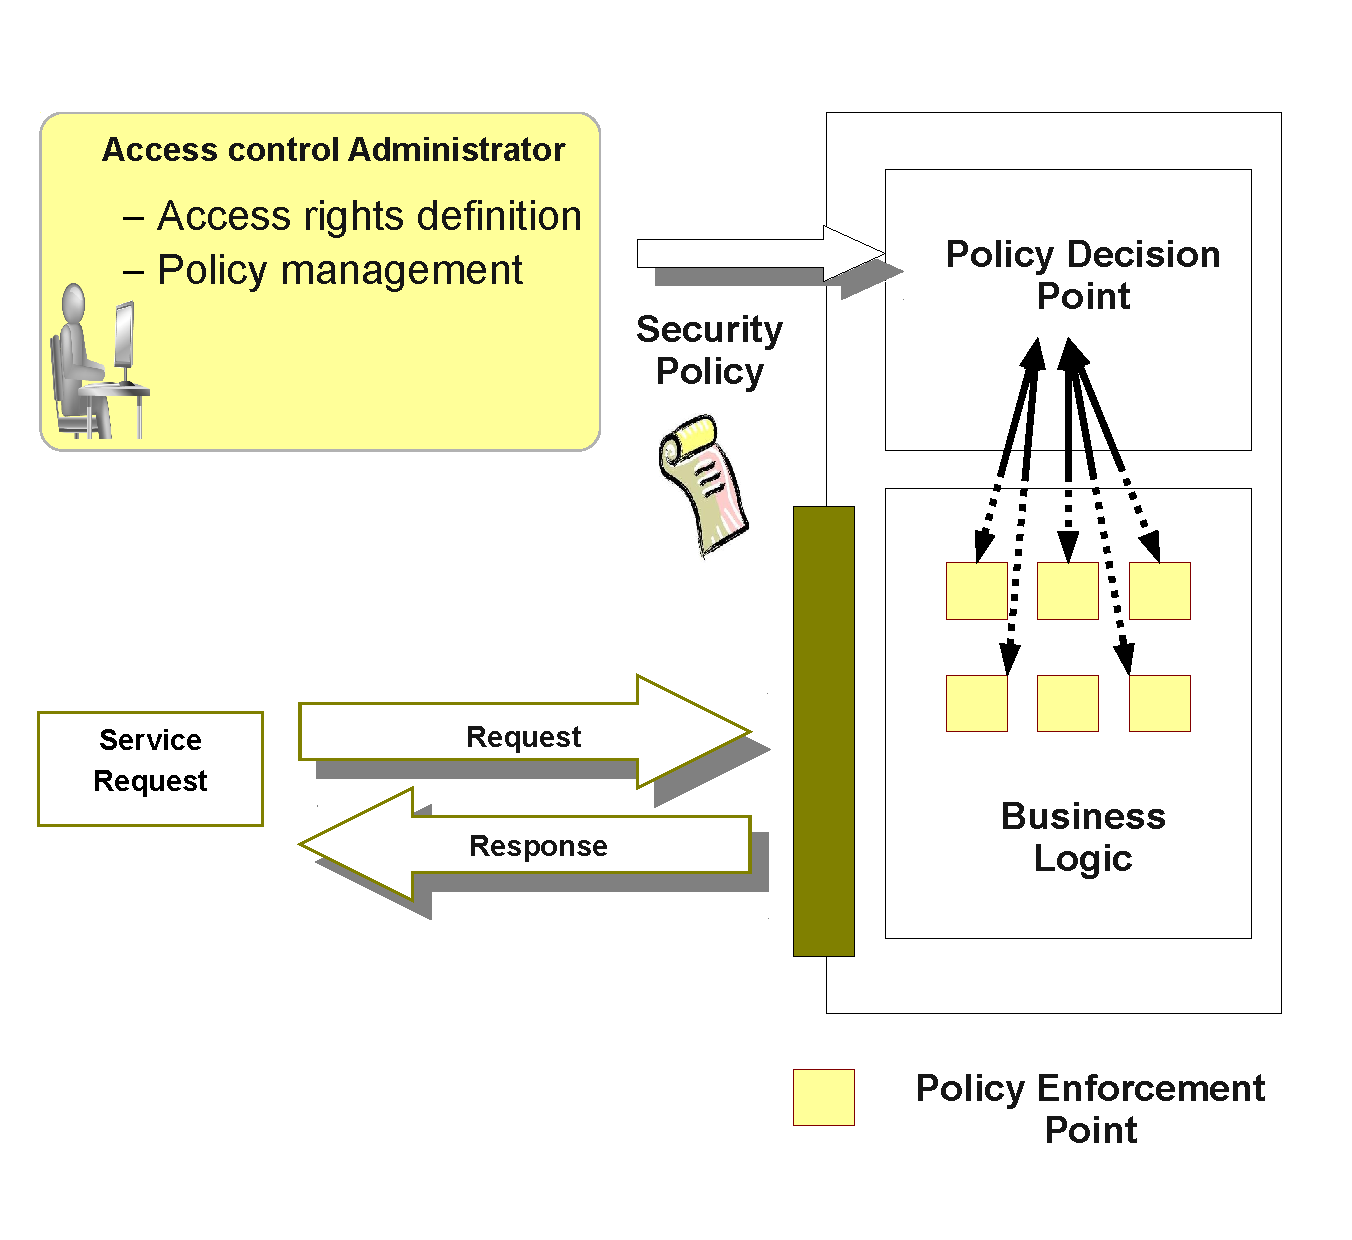
\includegraphics[width=9cm, height=8cm]{business-logic}
\caption{Access Control Request Processing}
\label{pep-pdp}
\end{center}
\end{figure}

\subsection{Centralization: A Threat for performances}
In such a system (Figure \ref{pep-pdp}), when the service execution requires an access control, the PEP calls the PDP to 
retrieve an authorization decision based on the PDP encapsulated policy. This authorization decision is made through the evaluation of rules in the policy. 
Subsequently, an authorization decision (permit/deny) is returned to the PEP. When a huge number of access requests are sent to the PDP, two bottlenecks cause a degradation of performances:
\begin{itemize}
 \item 1) all the access requests have to be managed through the same input channel of the PDP. 
 \item 2) the centralized PDP computes an access request by searching which rule is applicable among all the rules it contains.
\end{itemize}

The execution time for the treatment of a request is thus strongly related to:
\begin{itemize} 
\item the number of access rules the PDP contains as well as to the ordering of the rules into a PDP \cite{clustering}.
\item the workload (number of requests).
\end{itemize}
The execution time to treat one request depends on the size (number of rules) the PDP contains. For a given PDP size, the execution time  to treat requests increases linearly with the workload (number of requests). 
Our hypothesis is: the more rules a PDP contains, the higher the slope gradient of the execution time submitted to an increasing workload. 
 \textit{Hypothesis 1} validity is studied in section \ref{sec:experiment}.
As a consequence, one possibility to increase performances consists in splitting the centralized PDP into PDPs of smaller sizes. 


\subsection{Centralization allows a good synergy between PEPs and PDP}
Centralization offers a desirable feature by simplifying the routing of requests to the right PDP. 
Figure \ref{model} illustrates the model of the access control architecture. In this model, a set of business processes, which comply to users' needs, are encapsulated in a given business logic 
which is enforced by multiple PEPs. Conceptually, the decision is decoupled from the enforcement and involves a decision making process in which each PEP 
interacts with one single PDP. The keypoint concerns the cardinality linking PEPs to the PDP. While a PDP is potentially linked to many PEPs, any PEP is strictly linked to exactly one 
PDP (which is unique in the centralized model). 
Since there is only one PDP, the requests are all routed to this unique PDP. This means that no particular treatment is required to map a given PEP in the business logic to 
the corresponding PDP, embedding the requested access rule. Another advantage of this many-to-one association is the clear traceability between what has been specified by the 
policy at the decision level and the internal security mechanisms enforcing this policy at the business logic level. In such setting, 
when access control policies are updated or removed, the related PEPs can be easily located and removed. Thus the application is updated synchronously 
with the policy changes. We call this desirable property \textit{synergy} of the access control architecture: an access control architecture is said to be \textit{synergic} if any PEP always sends its requests  to the same PDP. 
As a consequence, splitting the centralized PDP into PDPs of smaller sizes may break this "synergy". In the following, we will consider various ways to split a centralized PDP into smaller PDPs. 
The related \textit{hypothesis 2} is: with comparable PDP sizes, the overall system will be more performant when the architecture is synergic. This hypothesis is questioned in 
section \ref{sec:experiment}.

\subsection{Tradeoff for refactoring a centralized architecture into a decentralized one}

As a synthesis for this section, the following facts are taken into account:
\begin{itemize}
 \item Access control architectures are centralized with a unique PDP
\item Centralization eases reconfiguration of access control policy
\item Centralization threatens performances
\item Direct mapping from any PEP to only one PDP makes the access control architecture "synergic"
\item A synergic system facilitates PEPs request routing and eases access control policy updates

\end{itemize}

The goal of this paper is to propose systematic ways to improve performance by refactoring the centralized model into a decentralized version, with multiple PDPs. The resulting
 architecture must be functionally equivalent and should not impact the desirable properties of the centralized model, namely reconfigurability and synergy.
Automating the transformation from a centralized to a decentralized architecture is required to preserve reconfigurability. With automation, we can still reconfigure the centralized policy, 
and then automatically refactor the architecture. Automated refactoring is thus a viable solution for having high reconfigurability.  
However, refactoring the architecture by splitting the centralized PDP into smaller one may break the initial synergy. This phenomenon is studied in the empirical study of section 
\ref{sec:experiment} together with \textit{hypothesis 2}. 
We describe the XACML Language since it is the standard language used to implement a PDP.


\begin{figure}[!h]
\begin{center}
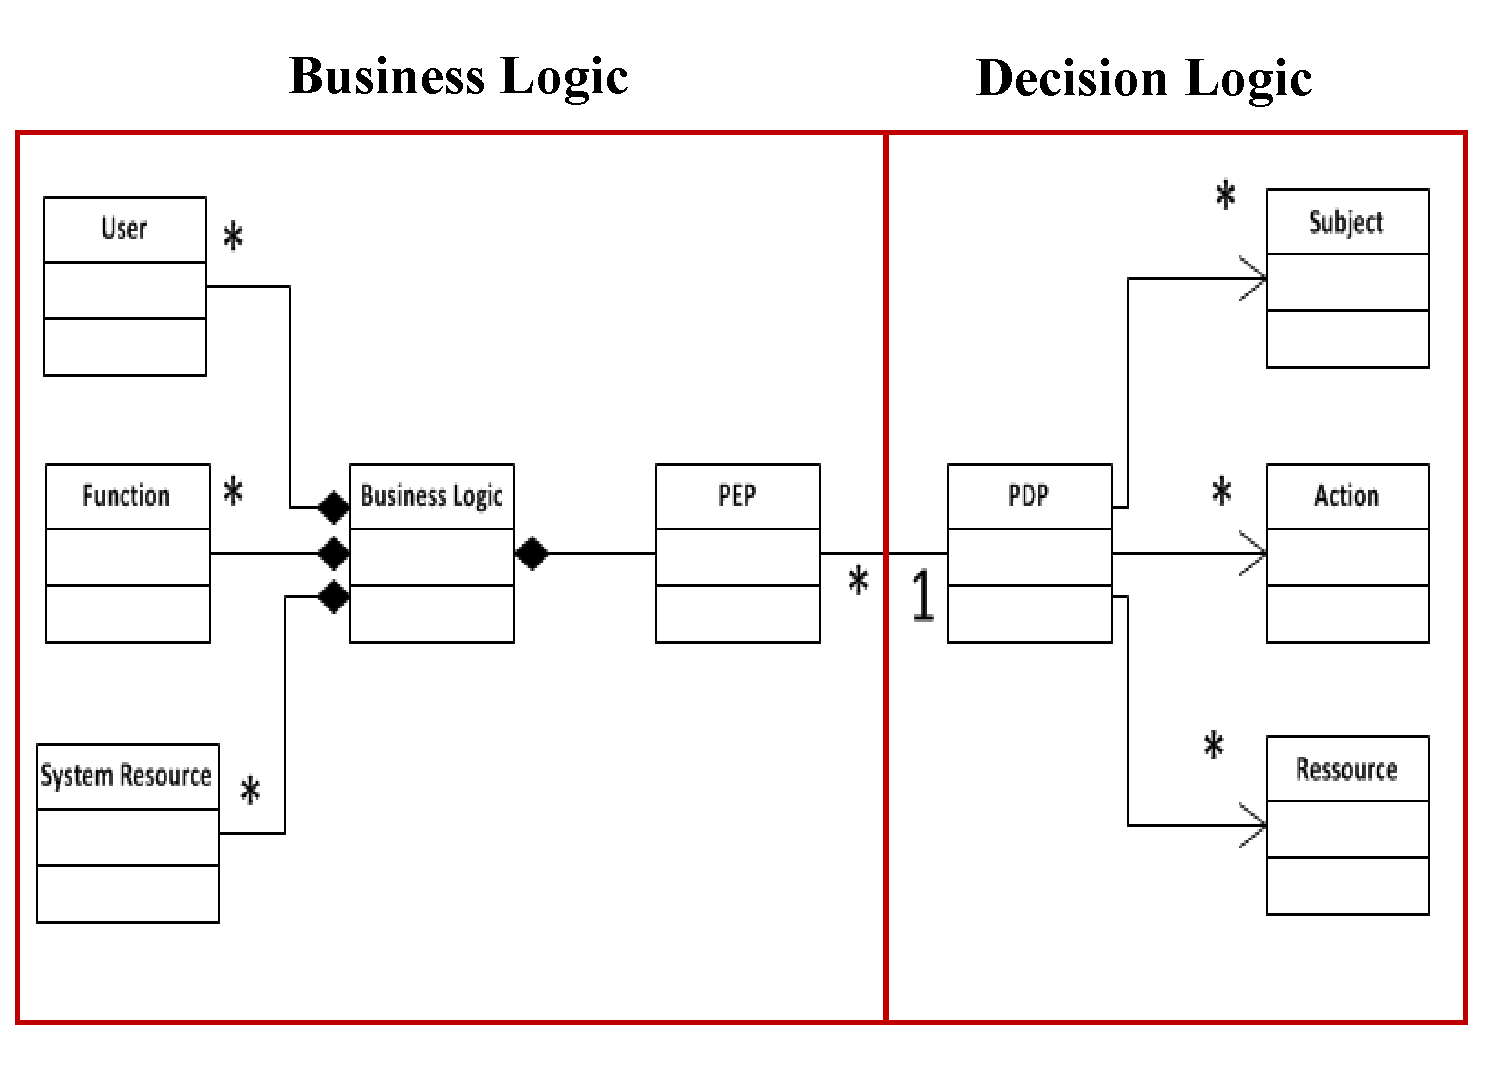
\includegraphics[height=5.5cm,width=8.5cm]{model}
\caption{The Access Control Model}
\label{model}
\end{center}
\end{figure}

\subsection{XACML Access Control Policies and Performance Issues}

In this paper, we focus on access control policies specified in the eXtensible Access Control Modeling Language (XACML) \cite{sunxacml}.
XACML is an XML-based standard policy specification language that defines a syntax of access control policies and
request/response. \\XACML enables policy authors to externalize access control policies for the sake of interoperability since access control policies can be designed 
independently from the underlying programming language or platform. Such flexibility enables to easily update access control policies to comply with new requirements.

An XACML is constructed as follows.
A \CodeIn{policy set} element consists of a sequence of \CodeIn{policy elements}, a combining algorithm, and
a \CodeIn{policy target} element. A \CodeIn{policy element} is expressed through a target, a set of \CodeIn{rules}, and a rule combining algorithm. 
A \CodeIn{target} element consists of the set of resources, subjects, and actions to which a rule is applicable. A \CodeIn{rule} consists of a 
\CodeIn{target} element, a \CodeIn{condition} element, and an \CodeIn{effect}. A \CodeIn{condition} element is a boolean expression that specifies the
environmental context (e.g., time and location restrictions) in which the rule applies.
Finally, an \CodeIn{effect} is the rule's authorization decision, which is either permit or deny.

Given a request, a PDP evaluates the request against the \CodeIn{rules} in the policy by matching resources, subjects, actions, and condition in the request.
More specifically, an XACML request encapsulates attributes, which define which subject requests to take action on which resource in which
condition (e.g., subject Bob requests to borrow a book).
%This can be under/not a condition.
Given a request, that satisfies \CodeIn{target} and \CodeIn{condition} elements in a rule, the rule's effect
is taken as the decision.
If the request does not satisfy \CodeIn{target} and \CodeIn{condition} elements in any rule, its response yields the ``NotApplicable'' decision.

When more than one rule is applicable to a request, the combining algorithm helps determine which rule's effect can be finally given as the decision for the request.
For example, given two rules, that are applicable to the same request and provide different decisions,
the permit-overrides algorithm prioritizes a permit decision over the other decisions.
More precisely, when using the permit-overrides algorithm, the policy evaluation produces one of the following three decisions: 

\begin{itemize}
\item Permit if at least one permit rule is applicable for a request.
\item Deny if no permit rule is applicable and at least one deny rule is applicable for a request.
\item NotApplicable if no rule is applicable for a request.
\end{itemize}

Figure \ref{figur1} shows a simplified XACML policy that denies subject Bob to borrow a book.

%\fontsize{5}{5}
\begin{figure}[!h]
\begin{center}
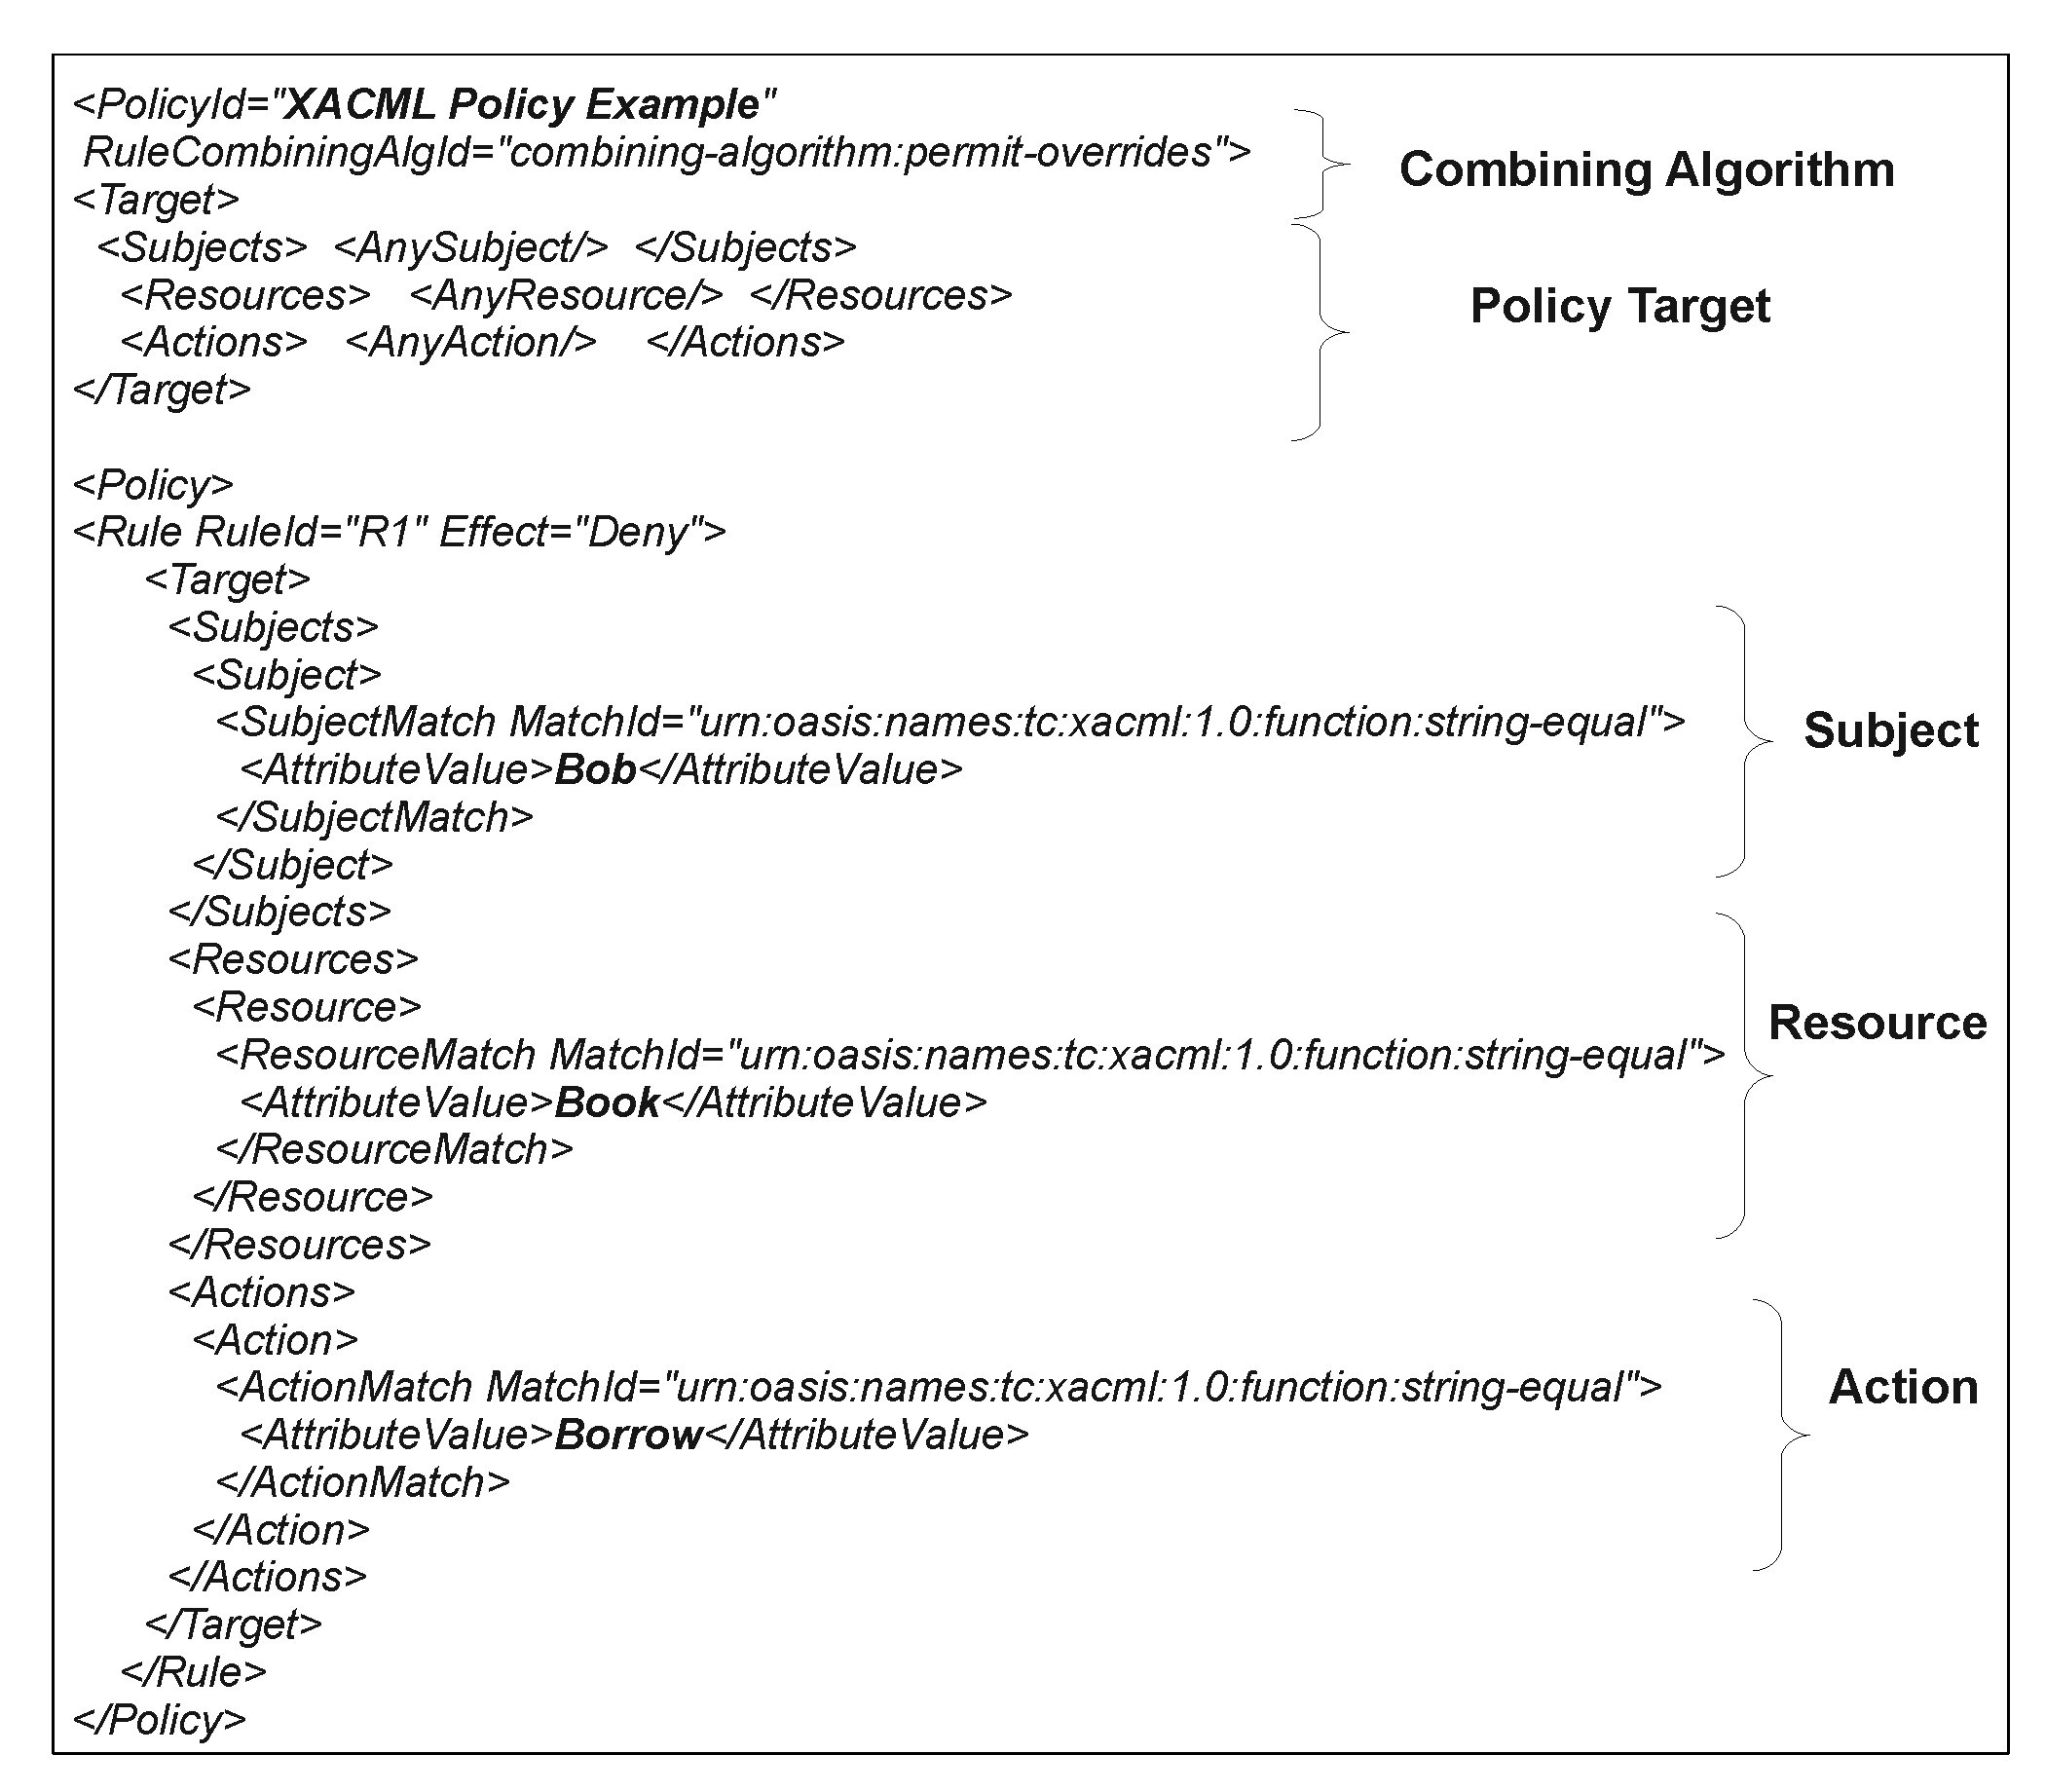
\includegraphics[width=8.6cm]{xacml}
\caption{XACML Policy Example}
\label{figur1}
\end{center}
\end{figure}

 
\Comment{ 
\begin{figure}[!h]%{t}
%\begin{figure}[firstnumber=100]
\begin{CodeOut}
\begin{alltt}
\small
 1 <PolicySet PolicyId="\textbf{An Example Policy Set}" PolicyCombAlgId="\textbf{Permit-overrides}">
 2 <Target/> 
 3  <Policy PolicyId="\textbf{An Example Policy}" RuleCombAlgId="\textbf{Permit-overrides}">
 4   <Target/>
 5    <Rule RuleId="\textbf{1}" Effect="\textbf{Deny}">
 6      <Target>
 7        <Subjects><Subject> \textbf{Bob} </Subject></Subjects>
 8        <Resources><Resource> \textbf{BOOK} </Resource></Resources>
 9        <Actions><Action> \textbf{BORROW} </Action></Actions>
10      </Target>
11	    <Condition>
12        <AttributeValue> \textbf{DEFAULT} </AttributeValue>
13      </Condition>
14    </Rule>
15      <!-- A final, "fall-through" rule that always Denies -->
16    <Rule RuleId="\textbf{FinalRule}" Effect="\textbf{Deny}"/>
17  </policy>
18 </policySet>
\end{alltt}
\end{CodeOut}
\vspace*{-3.0ex} \caption{An XACML Policy Example}
 \label{figur1}
\end{figure}
}
 

%\centering
%\figure[DREF metamodel\label{fig:drefMM}]
%        {\includegraphics[width=0.5\textwidth]{figure/drefMM}}
%\figure[SETER Process: Security Testing for Resilient Systems 
%\label{fig:seter}] {\includegraphics[width=0.49\textwidth]{figure/seter}}
%\caption{DREF and SETER: Conceptual and Operational Frameworks for evaluating resilient systems}
%\end{figure*}


Recently, an XACML policy becomes more complex to handle increasing complexity of organizations in terms of structure, relationships, activities, and access control requirements. In such a situation, the policy often consists of a large number of rules to specify policy behaviors for various resources, users and actions in the organizations.
In policy-based systems, policy authors manage centralized a single PDP loaded with a single policy to govern all of system resources. 
However, due to a large number of rules for evaluation, this centralization raises performance concerns related to request evaluation time for XACML access control policies and may 
degrade the system efficiency and slow down the overall business processes. 

We present following three main factors, that may cause to degrade XACML request evaluation performance: 

\begin{itemize}
\item An XACML policy may contain various attribute elements including \CodeIn{target} elements. Retrieval of
attribute values in the \CodeIn{target} elements for request evaluation may increase the evaluation time.
\item A \CodeIn{policy set} consists of a set of policies. Given a request, a PDP determines the final authorization decision (i.e., effect) of the whole \CodeIn{policy set} after combining all the applicable rules' decisions according to the request.
Computing and combining applicable rules' decisions contributes to increase the evaluation time.
\item \CodeIn{Condition} elements in rules can be complex because these elements are built from an arbitrary nesting of non-boolean functions and attributes. 
In such a situation, evaluating \CodeIn{condi-\\tion} elements may slow down request evaluation time.
\end{itemize}


\section{XACML Policy Refactoring Process} \label{sec:approach}
This section describes our approach of refactoring access control policies to improve performance by reducing the number of policy rules. 
For refactoring policies in a systematic way, we propose seven policy splitting criteria
based on attribute set. Moreover, we explain how to select the splitting criterion, which preserves the synergy requirement in the access control architecture. 

 


\subsection{Definition of Policy based Splitting Criteria}


Given a request, a PDP adopts brute force searching to find its decision
by evaluating the request against policy rules one by one until the PDP finds an evaluation decision.
For request evaluation processing, not of all the rules are applicable to the request.
In order words, only part of the rules (i.e., relevant rules) are applicable to the request and can contribute
to determine a final authorization decision.
We propose an approach to evaluate a request against only the relevant rules for a given request by refactoring
access control policies.
  
%Our approach is to split a single global policy into multiple policies based on attributes combination. 
Our approach refactors a policy into a set of sub-policies where the rules have the same values of attributes of subject, resource, or 
action.
Formally, our approach refactors an policy \normalsize $P$ into 
multiple policies \normalsize $P_{SC_{w}}$ based on Splitting Criteria $SC_{w}$.
These multiple policies contain less number of rules (compared to the number of rules in \normalsize $P$) and conforms to a Splitting Criteria $SC_{w}$. An $SC_{w}$ defines the set of attributes, which classify all of policy rules into subsets with the same attribute values for
selected attributes.
$w$ denotes the number of attributes that have to be considered conjointly for aggregating 
rules based on selected attributes. 


 
We first consider two attributes (e.g., $\langle Subject, Action\rangle$ or $\langle Action$, $Resource\rangle$) for Splitting Criteria. In such a setting, our approach refactors a policy into a set of 
policies each of which rules include the same couple of attribute elements. For example, $\langle Subject, Action\rangle$ criterion
classifies rules with same subjects and actions into sub-policies.
We also extend our Splitting Criteria by considering three attributes such as resource, action, and subject.
Table~\ref{table1} shows our proposed splitting criteria categories according to the attribute elements combination.

\begin{table}[h!]
\centering
\setlength{\extrarowheight}{6 pt}
\begin{tabular}{|>{\small}c|>{\small}c|} 
\hline  \rowcolor{black} 
\bf
\textcolor{white}{Categories}& \bf \textcolor{white}{Splitting Criteria}\\ \hline
$SC_{1}$& {$\langle Subject \rangle, \langle Resource\rangle, \langle Action\rangle$}\\ \hline
$SC_{2}$& {$\langle Subject,Action \rangle, \langle Subject,Resource\rangle$}\\&{$\langle Resource,Action\rangle$}\\  \hline
$SC_{3}$& {$\langle Subject,Resource,Action\rangle$}\\ \hline
\end{tabular}
\caption{Splitting Criteria}
\label{table1}\end{table}



Once the splitting process is performed, the access control architecture will include one or more (PDPs) that comply with a certain splitting criterion.
We use SUN PDP \cite{sunxacml} as a decision engine framework that evaluates requests against the policies specified in XACML.
During the evaluation process, SUN PDP checks the request against the policy and determines whether its authorization
decision is 
permit or deny. SUN PDP permits to load the considered policy in a file which is used during the decision making process, once the applicable policy 
is selected from this file, the decision engine fetches the policy to retrieve the applicable rules that are applicable to the request.


Figure \ref{requestevaluation} presents an evaluation process that considers resulting policies from the splitting process. 
During the evaluation process the applicable 
policy is selected from the configuration file. Sun's XACML enables to select the applicable policy, by verifying the matching between the request's attributes
 and the policy set attributes. 
After the selection of the applicable policy, all its rules which are considered relevant for the decision making are evaluated.

\begin{figure}[!h]
\begin{center}
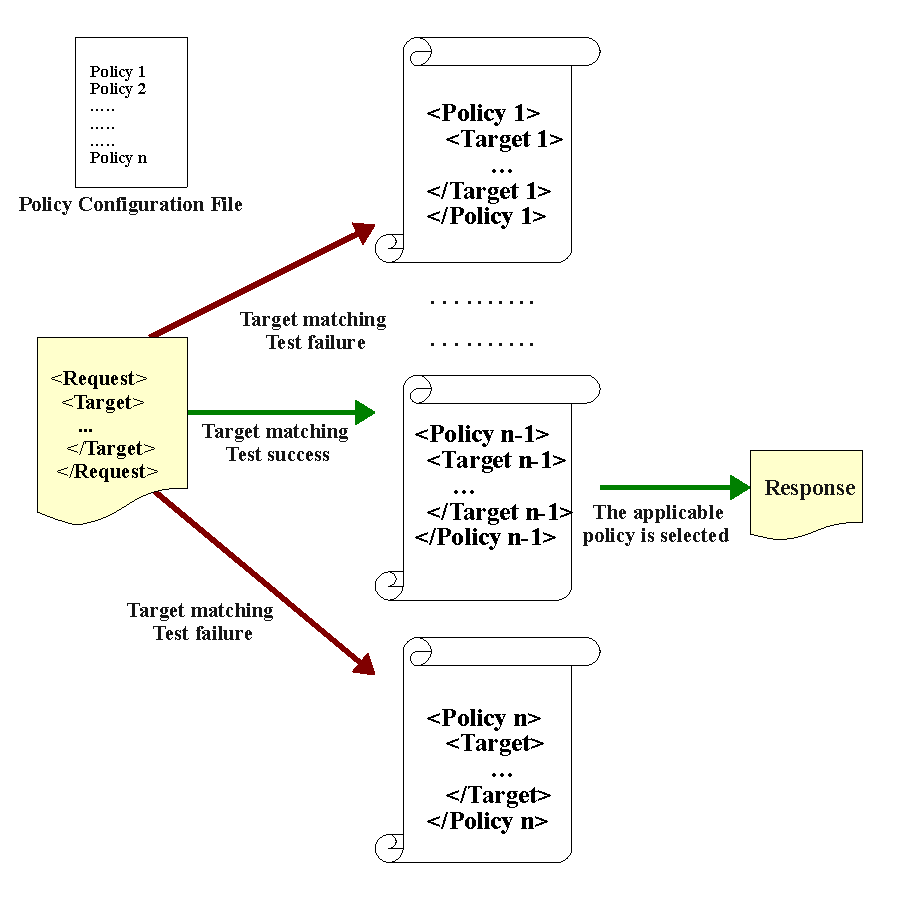
\includegraphics[width=3in, height=3in]{requestevaluation}
\caption{Applicable policy Selection}
\label{requestevaluation}
\end{center}
\end{figure}

As depicted in Figure \ref{overallprocess}, the refactoring process is automated and starts by specifying and creating the XACML file which 
will be split by our tool according to a specified SC that can be chosen by an access control stakeholder. Afterwards, the policies are included in the 
framework that supports our approach. For every change in the access control policy, the initial policy is updated and 
split again in order to be included again in the framework.
From a point of view of the system administration, maintaining and updating the access control policies is completely a standalone and simple
 process. The input is usually a centralized XACML policy. This input remains the same than before the access control performance issue is tackled.
Our process is transparent in the sense that it does not impact the existing functional aspects of the access control management system, 
for system administrators, who have to update the policy frequently and have to manage various dimensions of access control 
systems such the scalability and maintainability.
\begin{figure}[!h]
\begin{center}
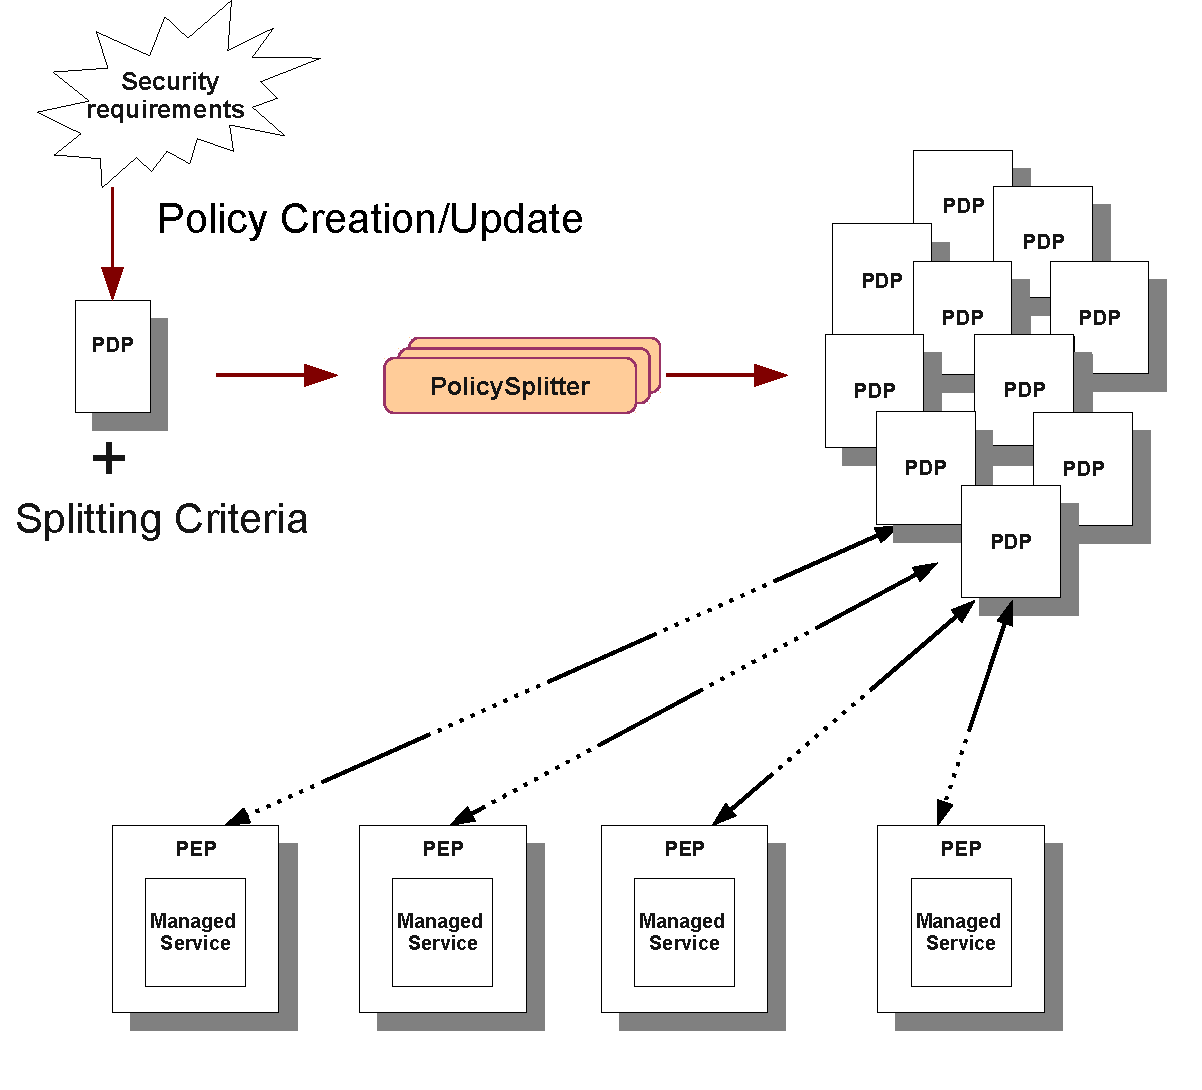
\includegraphics[width=8.5cm, height=8cm]{Overall-process}
\caption{Overview of the Refactoring Process}
\label{overallprocess}
\end{center}
\end{figure} 

To illustrate our approach, we present some examples that take into consideration the XACML language features:
\begin{itemize}
\item The refactoring of the XACML policy $P$ presented in Figure \ref{splitting} according to the splitting criterion $SC_{1}=\langle Subject\rangle$ consists in splitting $P$ 
into sub-policies $Pa$ and $Pb$ where each sub-policy groups the rules that are relevant to the same subject (Alice and Bob in this case). 

\item
XACML target elements may have an intricate structure, if they encapsulate the following elements $\langle Resou\-rceMatch\rangle$, $\langle SubjectMatch\rangle$, $\langle ActionMatch\rangle$.
These elements define a set of target elements related entities that match at the decision level with the context element in 
an access control request. In the example, shown in Figure\ref{xacml-match}, subject attribute includes two attributes (one is "role" and the other is "isEq-subjUserId-resUserId"). 
This subject can match with a request if the request has that at least role is pc-member and isEq-subjUserId-resUserId is true. In such configuration, the whole element subject is considered 
as a single entity that is not splitted by our supporting tool.

\item 

In XACML, policies and requests could be multi-valued. For example, the subject in a given request could both be the manager and the employee as a principal.
For the sake of simplicity, we don't consider multi-valued requests in this work.
\end{itemize}
\begin{figure}[!h]
\begin{center}
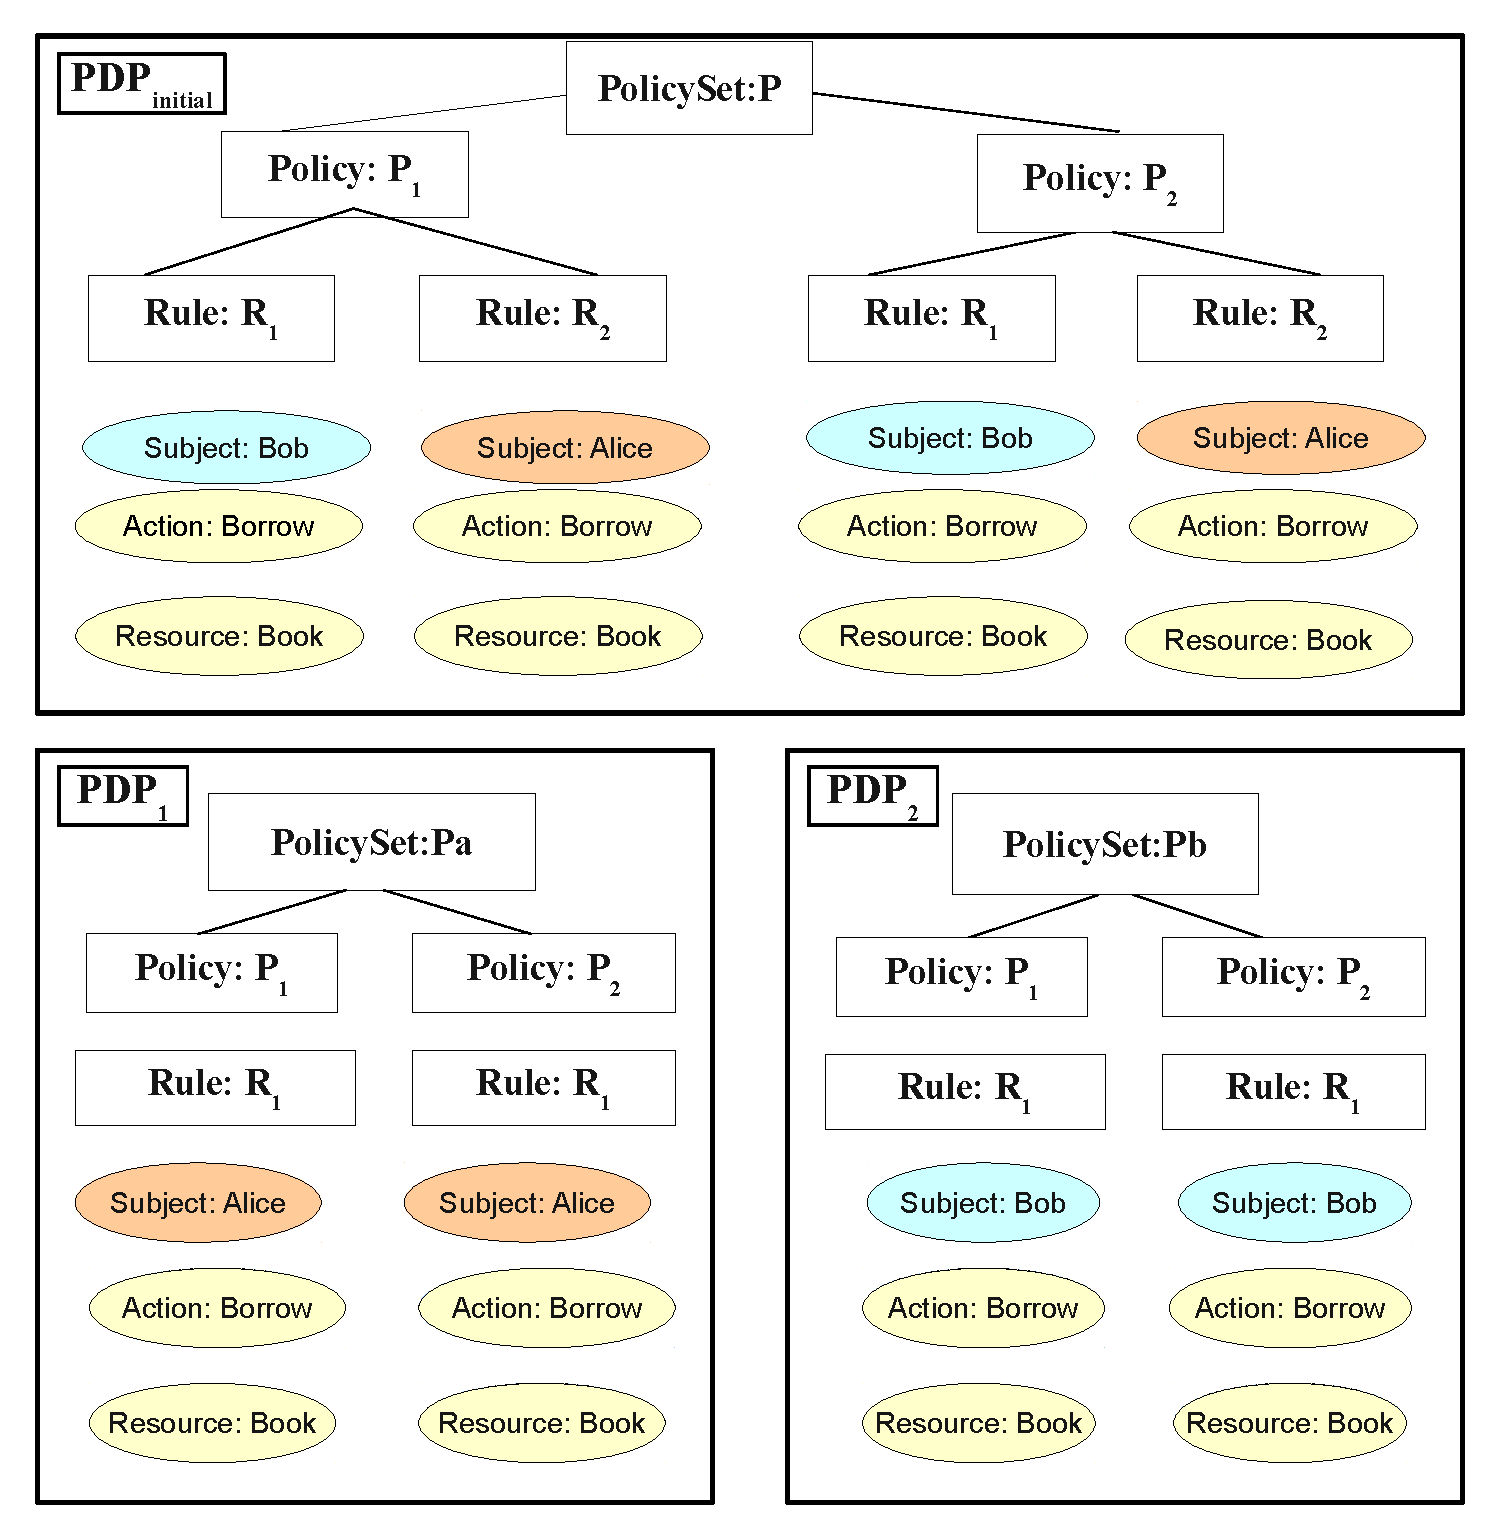
\includegraphics[width=8.5cm, height=7cm]{splitting}
\caption{Splitting a Policy according to $SC_{1}=\langle Subject\rangle$}
\label{splitting}
\end{center}
\end{figure} 


\begin{figure}[!h]
\begin{center}
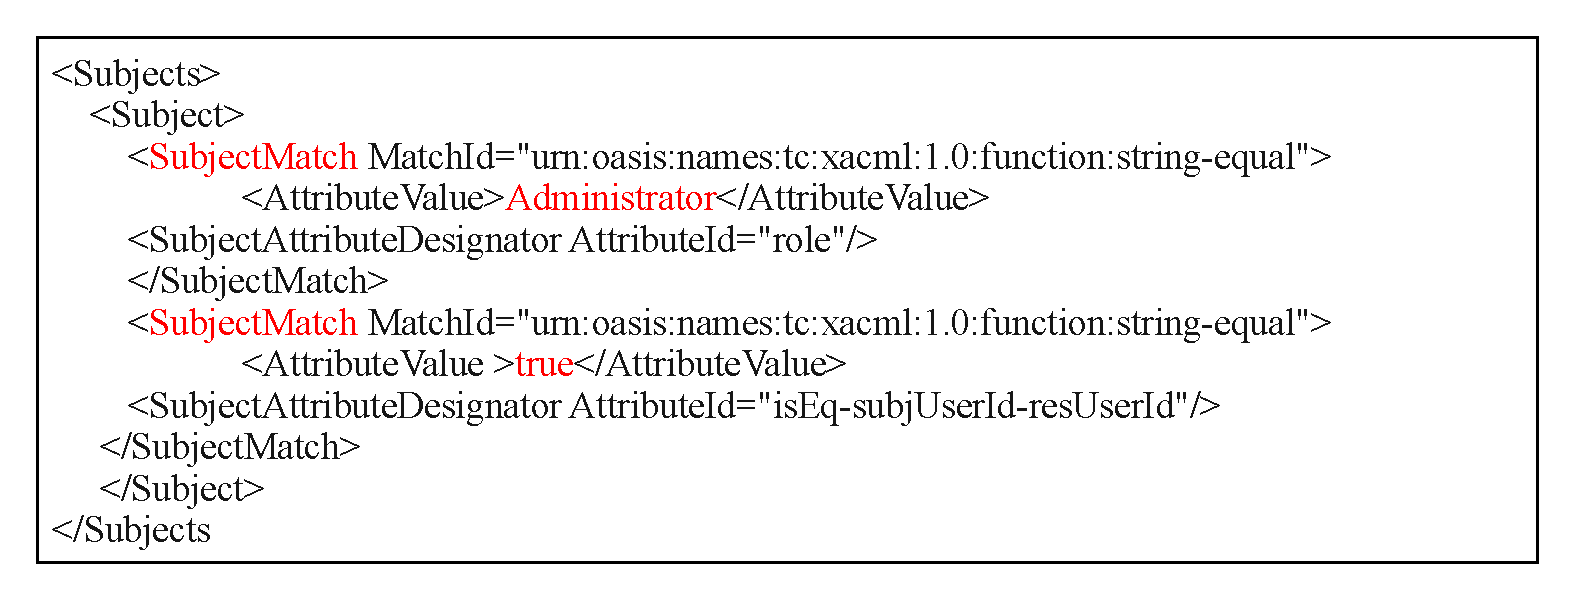
\includegraphics[width=9cm, height=3.5cm]{xacml-match}
\caption{Multi-attributes values Target Element}
\label{xacml-match}
\end{center}
\end{figure}
 


\subsection{Architecture Model Preservation: PEP-PDP Synergy}
We consider the different splitting criteria that we have identified in the previous section and we propose to select the splitting criterion that 
enables to preserve the synergy requirement in the access control architecture, this splitting criterion enables to have a valid refactoring and respects how PEPs are organized 
at the application level and how they are linked to their corresponding PDPs.

In the worst case, splitting the initial PDP into multi-PDPs may lead to a non-synergic system: a PEP may send its requests to several PDPs. 
The PDP, which receives a request is only known at runtime. Such a resulting architecture breaks the PEP-PDP synergy and the conceptual 
simplicity of the initial architecture model. In the best case, the refactoring preserves the simplicity of the initial architecture, by keeping a many-to-one association 
from PEPs to PDPs. A given request evaluation triggered by one PEP will always be handled by the same PDP. Operationally, the request evaluation process will involve 
one XACML policy file. In this case, the refactoring is valid, since its does not impact the conceptual architecture of the system.

A deep analysis of the PEPs at the application enables to observe the mapping between the PEPs and the PDP. At the application level, the PEP
is represented by a method call that triggers a decision making process by activating some specific rules in the PDP.
The code in Figure \ref{PEP deployment Example} is taken from \cite{legacy}, this code excerpt shows an example of a PEP represented by the method checkSecurity which calls the class 
SecurityPolicyService that initiates the PDP component.
\begin{figure}[!h]
\begin{center}
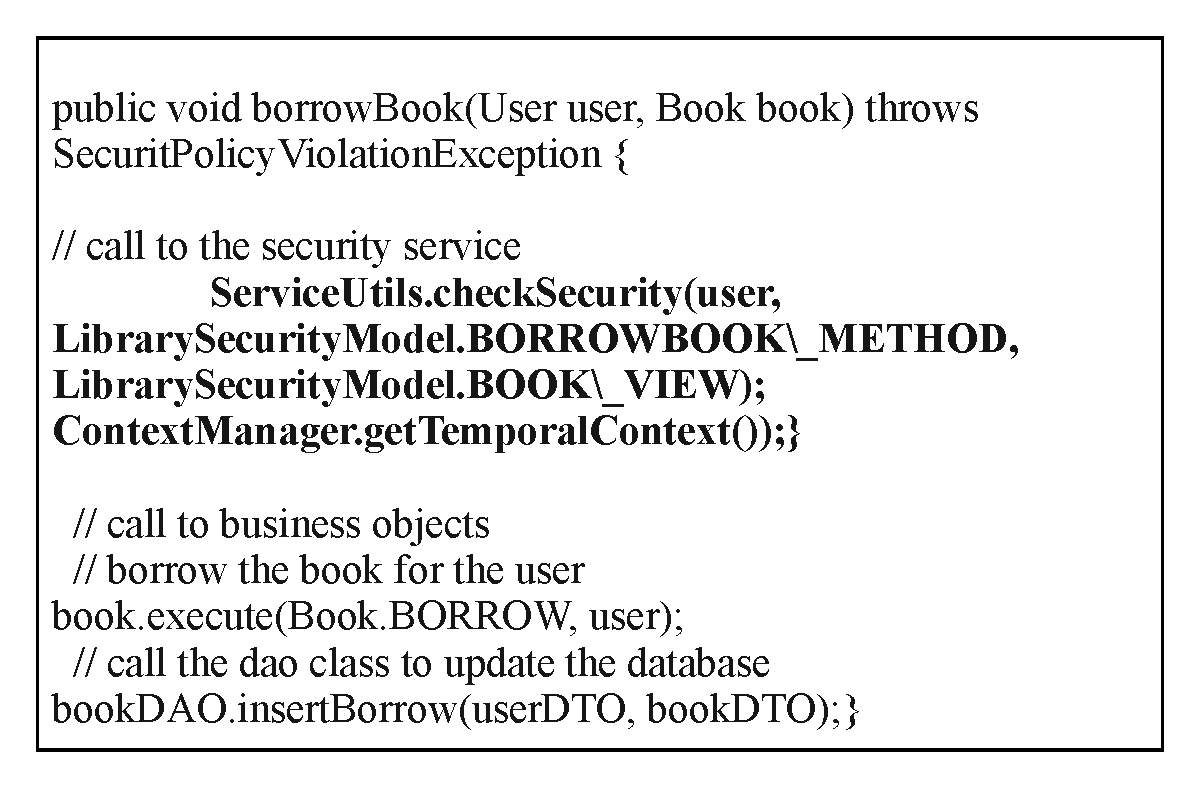
\includegraphics[width=7.5cm, height=4cm]{PEPExample}
\caption{PEP deployment Example}
\label{PEP deployment Example}
\end{center}
\end{figure}

An analysis of this code reflects that the PEP presented by the method ServiceUtils.checkSecurity will trigger exclusively all the rules 
that have the subject user (provided as input parameter in the PEP) and fixed Action and Resource (LibrarySecurityModel.BORROWBOOK\_METHOD), ( LibrarySecurityModel.BOOK\_VIEW).
Thus the splitting process that will preserve the mapping between the PEPs and the PDP is $SC_{2}=\langle Resource,Action\rangle$ since the rules in the policy are triggered 
by Action, Resource. Depending on the organization of the PEPs in a given application, connecting the rules with their PEPs at the application level may require to identify
 all the enforcements points in the application, and to track the different method calls triggered from these specific enforcement calls to map them to the relevant access control rules.

Our empirical results, presented in section~\ref{sec:experiment}, have shown that adopting a policy refactoring based on system functions, as a refactoring strategy, enables to 
have the best splitting criterion in term of performance. 
In this work we consider 3 evaluation studies where the PEPs trigger fixed couples of (action, resource) for variable subjects in the policies, thus the splitting criteria $SC_{2}=\langle Resource,Action\rangle$ is considered as 
the best splitting criteria that enables to preserve the synergy requirement in the architectural model. Inferring automatically the PEPs from the application enables to identify automatically
 for a given application the best splitting criteria, this can be easily applied using the testing technique presented in \cite{legacy}.


%\section{Experiment}\label{sec:experiment}
\section{Empirical results} \label{sec:experiment}
To measure the efficiency of our approach, we conducted two empirical studies. The first takes into consideration the whole system 
(PEPs and PDPs) to evaluate the performance improvement regarding the decision making process. The request processing time, 
for each splitting criterion is compared to the processing time of the initial architecture implementing the global policy (the evaluation 
that considers the global policy, is denoted (IA), the ``Initial Architecture''). The second empirical study focuses only on the PDPs in isolation to measure the gain in performance
 independently from the system. To make such study of PDPs in isolation, we use XEngine \cite{Xengine}. The objective of the second study is to see how our approach can be 
combined with XEngine and how this impacts the performance. The first subsection introduces our empirical studies and presents the tool that supports our approach. The remaining two 
sections present and discuss the results of the two empirical studies.  

\subsection{Empirical Studies and PolicySplitter Tool}
The empirical studies were conducted using the following systems \cite{testcase}:
\begin{itemize}	
\item LMS: The library management system offers services to manage books in a public library.
\item VMS: The virtual meeting system offers simplified web conference services. The virtual meeting server allows the organization of work meetings on 
a distributed platform.
\item ASMS (Auction Sale Management System): allows users to buy or sell items online. A seller can start an auction by submitting a description of the
item he wants to sell and a minimum price (with a start date and an ending date for the auction). Then usual bidding process can apply and people can bid 
on this auction. One of the specificities of this system is that a buyer must have enough money in his account before bidding.
\end{itemize}
We completed the set of existing rules with all implicit rules that were not explicitely originally described. This provides a larger set of access rules that enables
an accurate comparison of performances. As a result, LMS policy contains 720 rules, 
VMS has 945 rules while ASMS implements 1760 rules. 
Our evaluations were carried out on a desktop PC, 
running Ubuntu 10.04 with Core i5, 2530 Mhz processor, and 4 GB of RAM. 
We have implemented the PolicySplitter tool in Java. PolicySplitter enables splitting the policies according to the chosen splitting criteria. 
The tool is available for download from \cite{splitter}.
The execution time of the tool is not considered as a performance factor as it takes up to few seconds (for very large policies) to perform the splitting 
according to all SCs. Moreover the refactoring process is executed only once to create a configuration that supports a selected splitting criterion.


\subsection{Performance Improvement Results}
For the 3 evaluation studies, we generated the resulting sub-policies for all the splitting criteria that we have defined in Section III.
The decision Engine in our three case studies is based on Sun XACML PDP implementation \cite{sunxacml}. We choose to use Sun XACML PDP instead of XEngine in order 
to prove the effectiveness of our approach when compared to the traditional architecture.
% To run the experiments, we used a configuartion file that maintains the list of policies used for requests evaluation. 
% For the initial architecture, the configuration file contains one policy. Sun XACML PDP uses this configuration file to select to XACML files that constitute the policy.
For each splitting criteria, we have conducted systems tests to generate 
requests that trigger all the PEPs in the three evaluation studies. The test generation step leads to the execution of all combination of possible requests, 
all the details related to this step are presented in details in our previous \cite{testcase}.
  
The process of tests generation is repeated ten times in order to avoid the impact of randomness.
We applied this process to each splitting criterion and calculated the average execution time.


% We only consider the execution time of the PDP and we do not include the executions of the system functions. 
The results are shown in Figure \ref{fig:processing time}. They show the execution time considering the sub-policies resulting from each splitting criterion and the global policy 
that corresponds to the initial architecture (IA). Note that the results are ranked from the largest processing duration to the smallest one. 
From the Figure \ref{fig:processing time}, we can make two observations:

\begin{itemize} 
\item Compared to the initial architecture (IA), the evaluation time is considerably reduced for all the splitting criteria. This is consistent with our 
initial intuition. In fact, splitting the policy into small policies improves requests processing duration.
\item The splitting criteria \normalsize $SC=\langle Action, Resource\rangle$ enables to have the best evaluation time. 
In fact, the PEPs in the 3 empirical studies are scattered across the applications by a categorization 
that is based on $\langle Action, Resource\rangle$. This pleads in favor of adopting a splitting criteria that takes into account the PEP-PDP synergy requirement.
\end{itemize} 
\begin{figure*}
  \centering
  \subfloat[LMS]{\label{fig:gull}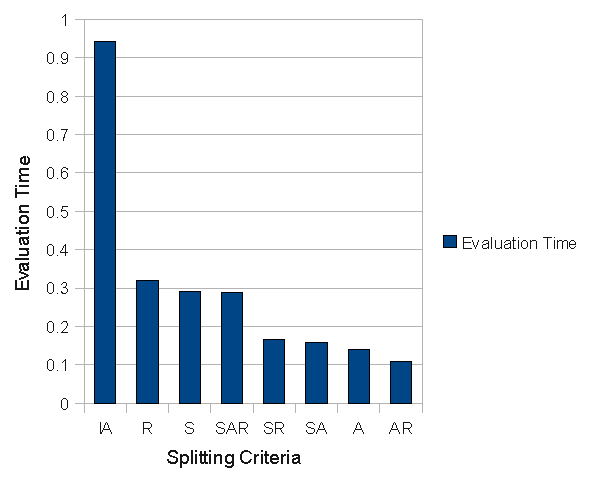
\includegraphics[width=0.33\textwidth]{LMS.pdf}}                
  \subfloat[VMS]{\label{fig:VMS}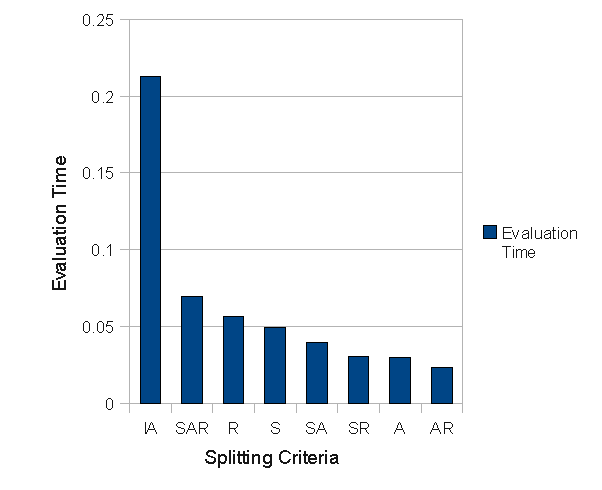
\includegraphics[width=0.33\textwidth]{VMS.pdf}}
  \subfloat[ASMS]{\label{fig:ASMS}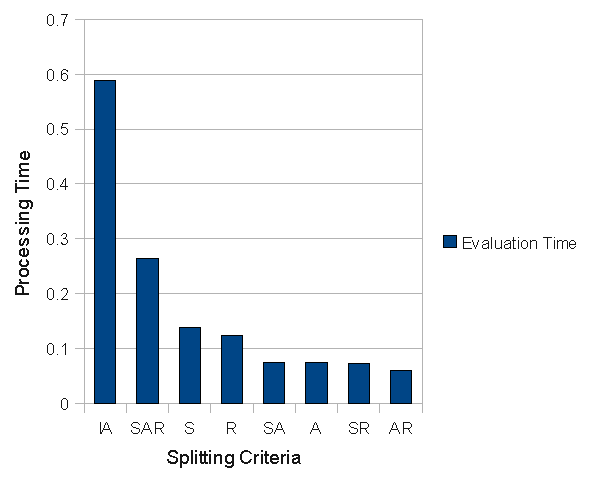
\includegraphics[width=0.33\textwidth]{ASMS.pdf}}
  \caption{Processing Time for our 3 systems LMS, VMS and ASMS}
  \label{fig:processing time}
\end{figure*}
\begin{figure}[!h]
  \centering
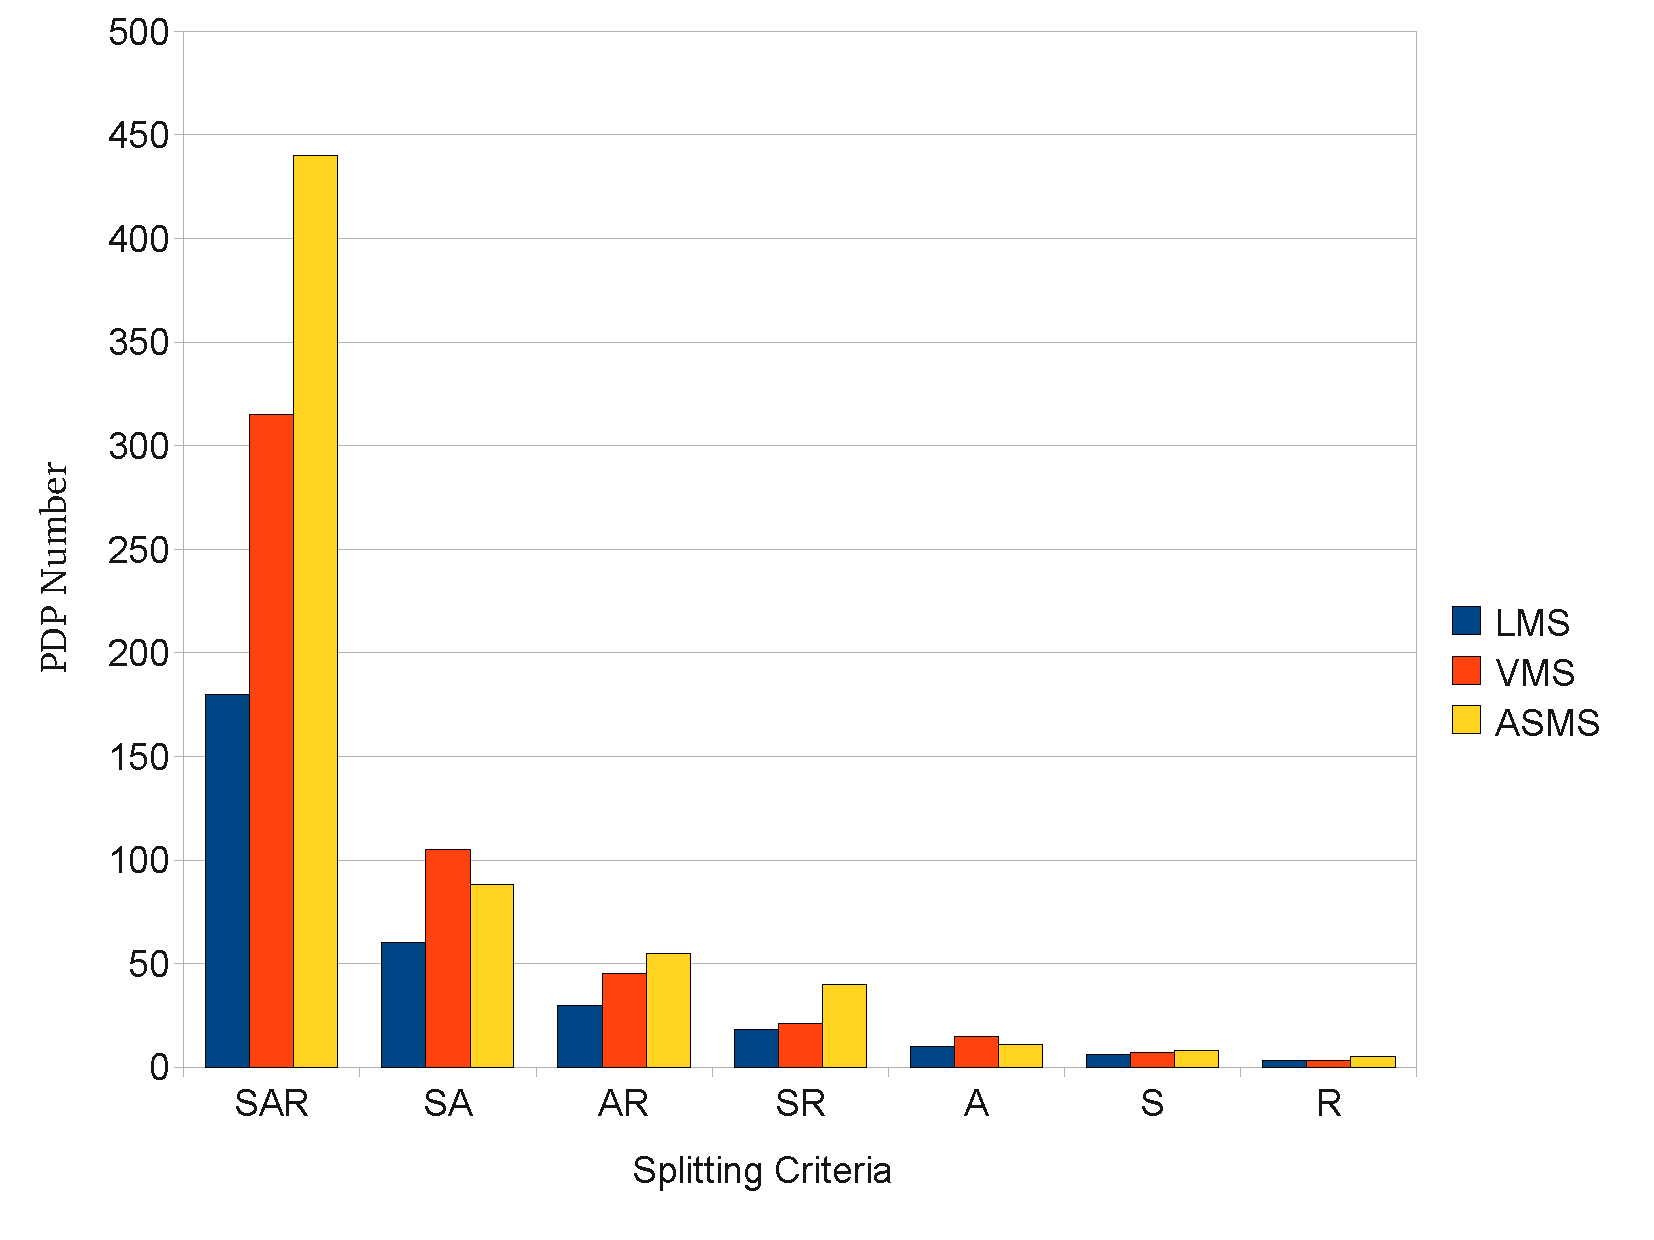
\includegraphics[width=8.5cm, height=7.2cm]{pdpnumber.pdf}
\begin{center}
\caption{PDP Number According to Splitting Criteria}
\label{pdpnumber}
\end{center}
\end{figure} 

In a second step, we have evaluated PDPs number generated by each splitting criterion, to study the impact of the refactoring process on the initial policy. 
For the 3 XACML studies, we executed the PoliySplitter tool on the 3 initial policies and we generated the number of resulting policies, in each study. 
As highlighted by Figure \ref{pdpnumber}, we notice that there are three
 categories of results: $SC_{1}$ category leads to a small number of PDPs, $SC_{2}$ category produces a reasonable number of PDPs whereas $SC_{3}$ leads to a huge 
number of PDPs. $SC_{2}$ category, thus appears as a good tradeoff in terms of performance and number of 
PDPs generated: In our evaluation studies, $SC=\langle Action, Resource\rangle$ is the best criterion, both in terms of performances and low number of PDPs.


\subsubsection{Performance improvement with XEngine}
The goal of this empirical study is to show the impact of combining XEngine as a decision engine rather than Sun XACML PDP implementation with our approach. 
We have chosen to use \cite{Xengine}, mainly for 3 reasons:

\begin{itemize}
\item It uses a refactoring process that transforms the hierarchical structure of the XACML policy to a flat structure. 
\item It converts multiple combining algorithms to single one.
\item It lies on a tree structure that minimizes the request processing time.
\end{itemize}
We propose to use XEngine conjointly with the refactoring process presented in this work:
We have evaluated our approach in 2 settings:
\begin{itemize}
\item Considering evaluations with a decision engine, based on SUN PDP, with split policies and with the initial policy.  
\item Considering evaluations with a decision engine, based on XEngine rather than Sun PDP, with split policies and with the initial policy as well.  
\end{itemize}

We have measured the processing time (in ms) of a randomly generated set of 10,000 requests. For request generation, we have used the technique presented 
in \cite{request}. The request time processing is evaluated for LMS, VMS, ASMS. The results are presented in Table I, II and III.

\begin{table}[h!]
\centering
\begin{tabular}{|>{\tiny}c|>{\tiny}c|>{\tiny}c|>{\tiny}c|>{\tiny}c|>{\tiny}c|>{\tiny}c|>{\tiny}c|>{\tiny}c|}   
\hline  \rowcolor{black} \scriptsize \bf \textcolor {white}{}
& \scriptsize \bf \textcolor {white}{SAR}
& \scriptsize \bf \textcolor {white}{AR}
& \scriptsize \bf \textcolor  {white}{SA}
& \scriptsize \bf \textcolor  {white}{SR}
& \scriptsize \bf \textcolor  {white}{R}

& \scriptsize \bf \textcolor  {white}{S} 
& \scriptsize \bf \textcolor  {white}{A}
& \scriptsize \bf \textcolor {white}{IA}\\ \hline
\scriptsize  {SUN }
&\scriptsize  {485}
& \scriptsize {922}
& \scriptsize {1453}
& \scriptsize {1875}
& \scriptsize {2578}

& \scriptsize {2703}
& \scriptsize {2703}
& \scriptsize {2625}
  \\ \hline
\scriptsize  {XEn}
&\scriptsize  {26}
& \scriptsize {47}
& \scriptsize {67}
& \scriptsize {95}
& \scriptsize {190}

& \scriptsize {164}
& \scriptsize {120}
& \scriptsize {613}
  \\ \hline
\end{tabular}
\caption{Evaluation time in LMS}\end{table}



\begin{table}[h!]
\centering
\begin{tabular}{|l|l|l|l|l|l|l|l|l|}   
\hline  \rowcolor{black} \scriptsize \bf \textcolor {white}{}
& \scriptsize \bf \textcolor {white}{SAR}
& \scriptsize \bf \textcolor {white}{AR}
& \scriptsize \bf \textcolor  {white}{SA}
& \scriptsize \bf \textcolor  {white}{SR}
& \scriptsize \bf \textcolor  {white}{R}

& \scriptsize \bf \textcolor  {white}{S} 
& \scriptsize \bf \textcolor  {white}{A}

& \scriptsize \bf \textcolor {white}{IA}\\ \hline

\scriptsize  {SUN }
& \scriptsize  {1281}
& \scriptsize {2640}
& \scriptsize {3422}
& \scriptsize {3734}
& \scriptsize {6078}

& \scriptsize {5921}
& \scriptsize {6781}
& \scriptsize {5766}
  \\ \hline
\scriptsize  {XEn}
& \scriptsize  {34}
& \scriptsize {67}
& \scriptsize {96}
& \scriptsize {145}
& \scriptsize {384}

& \scriptsize {274}
& \scriptsize {149}
& \scriptsize {265}
  \\ \hline
\end{tabular}
\caption{Evaluation time in VMS}\end{table}

\begin{table}[h!]
\centering
\begin{tabular}{|l|l|l|l|l|l|l|l|l|}   
\hline  \rowcolor{black} \scriptsize \bf \textcolor {white}{}
& \scriptsize \bf \textcolor {white}{SAR}
& \scriptsize \bf \textcolor {white}{AR}
& \scriptsize \bf \textcolor  {white}{SA}
& \scriptsize \bf \textcolor  {white}{SR}
& \scriptsize \bf \textcolor  {white}{R}

& \scriptsize \bf \textcolor  {white}{S} 
& \scriptsize \bf \textcolor  {white}{A}
& \scriptsize \bf \textcolor {white}{IA}\\ \hline
\scriptsize  {SUN }
& \scriptsize  {2280}
& \scriptsize {2734}
& \scriptsize {3625}
& \scriptsize {8297}
& \scriptsize {7750}

& \scriptsize {8188}
& \scriptsize {6859}
& \scriptsize {7156}
  \\ \hline
\scriptsize  {XEn}
& \scriptsize  {49}
& \scriptsize {60}
& \scriptsize {104}
& \scriptsize {196}
& \scriptsize {310}

& \scriptsize {566}
& \scriptsize {262}
& \scriptsize {1639}
  \\ \hline
\end{tabular}
\caption{Evaluation time in ASMS}\end{table}


From the different tables, we can observe that, when used with a decision engine based on XEngine rather than Sun PDP, our proposed approach provides more performance improvement. 
This empirical observation pleads in favour of applying our proposed refactoring process with XEngine.\\

In a second step, we have considered the workload of the software system. We evaluated the request procesing time according to the number of requests incoming to the system. 
For each policy in the three systems (ASMS, LMS, and VMS), we generate successively 5000, 10000,..,50000 random requests to measure the evaluation time (ms).
The results are shown in (reference to tables). For the three systems, we notice that the evaluation time increases when the number of requests increases in the system. 
Moreover, the request evaluation time is considerably improved when using the splitting process compared to the initial architecture.

\begin{figure*}
  \centering
  \subfloat[LMS]{\label{fig:gull}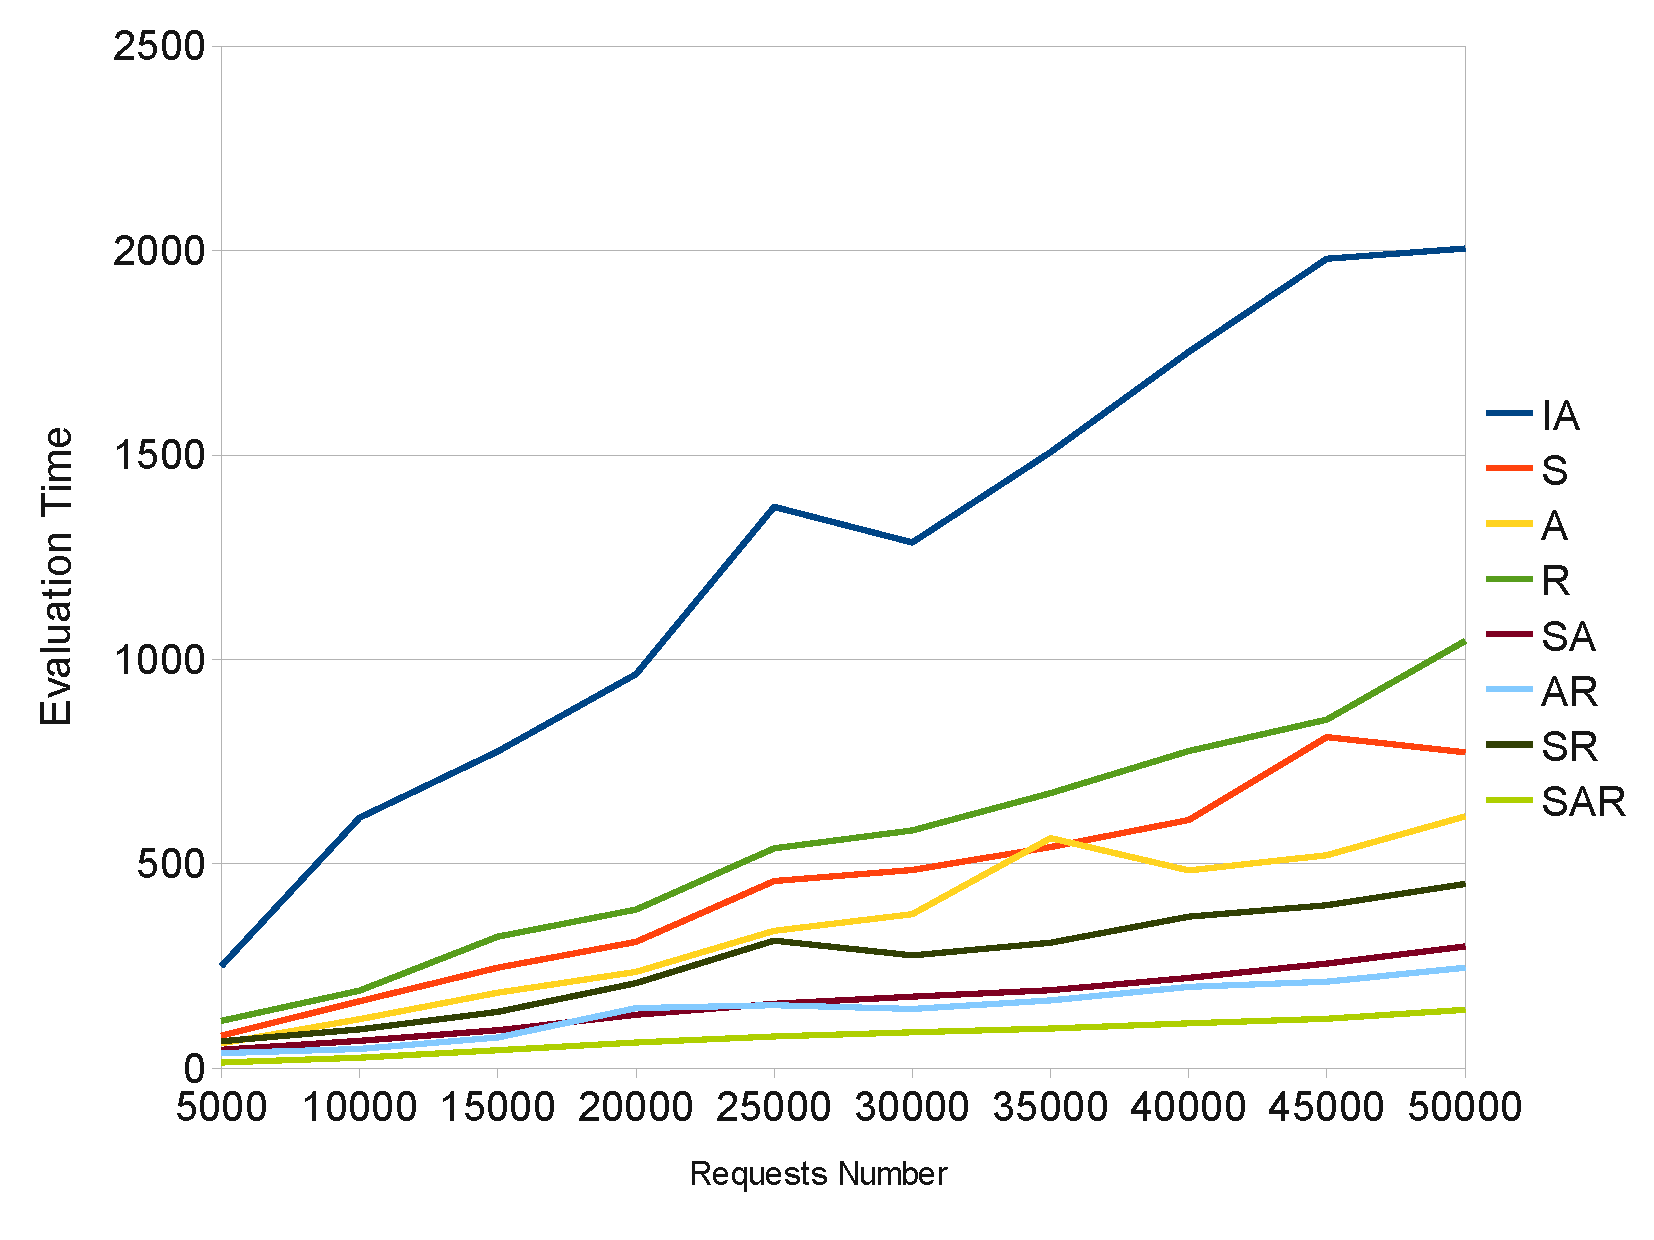
\includegraphics[width=0.33\textwidth]{X-LMS.pdf}}                
  \subfloat[VMS]{\label{fig:VMS}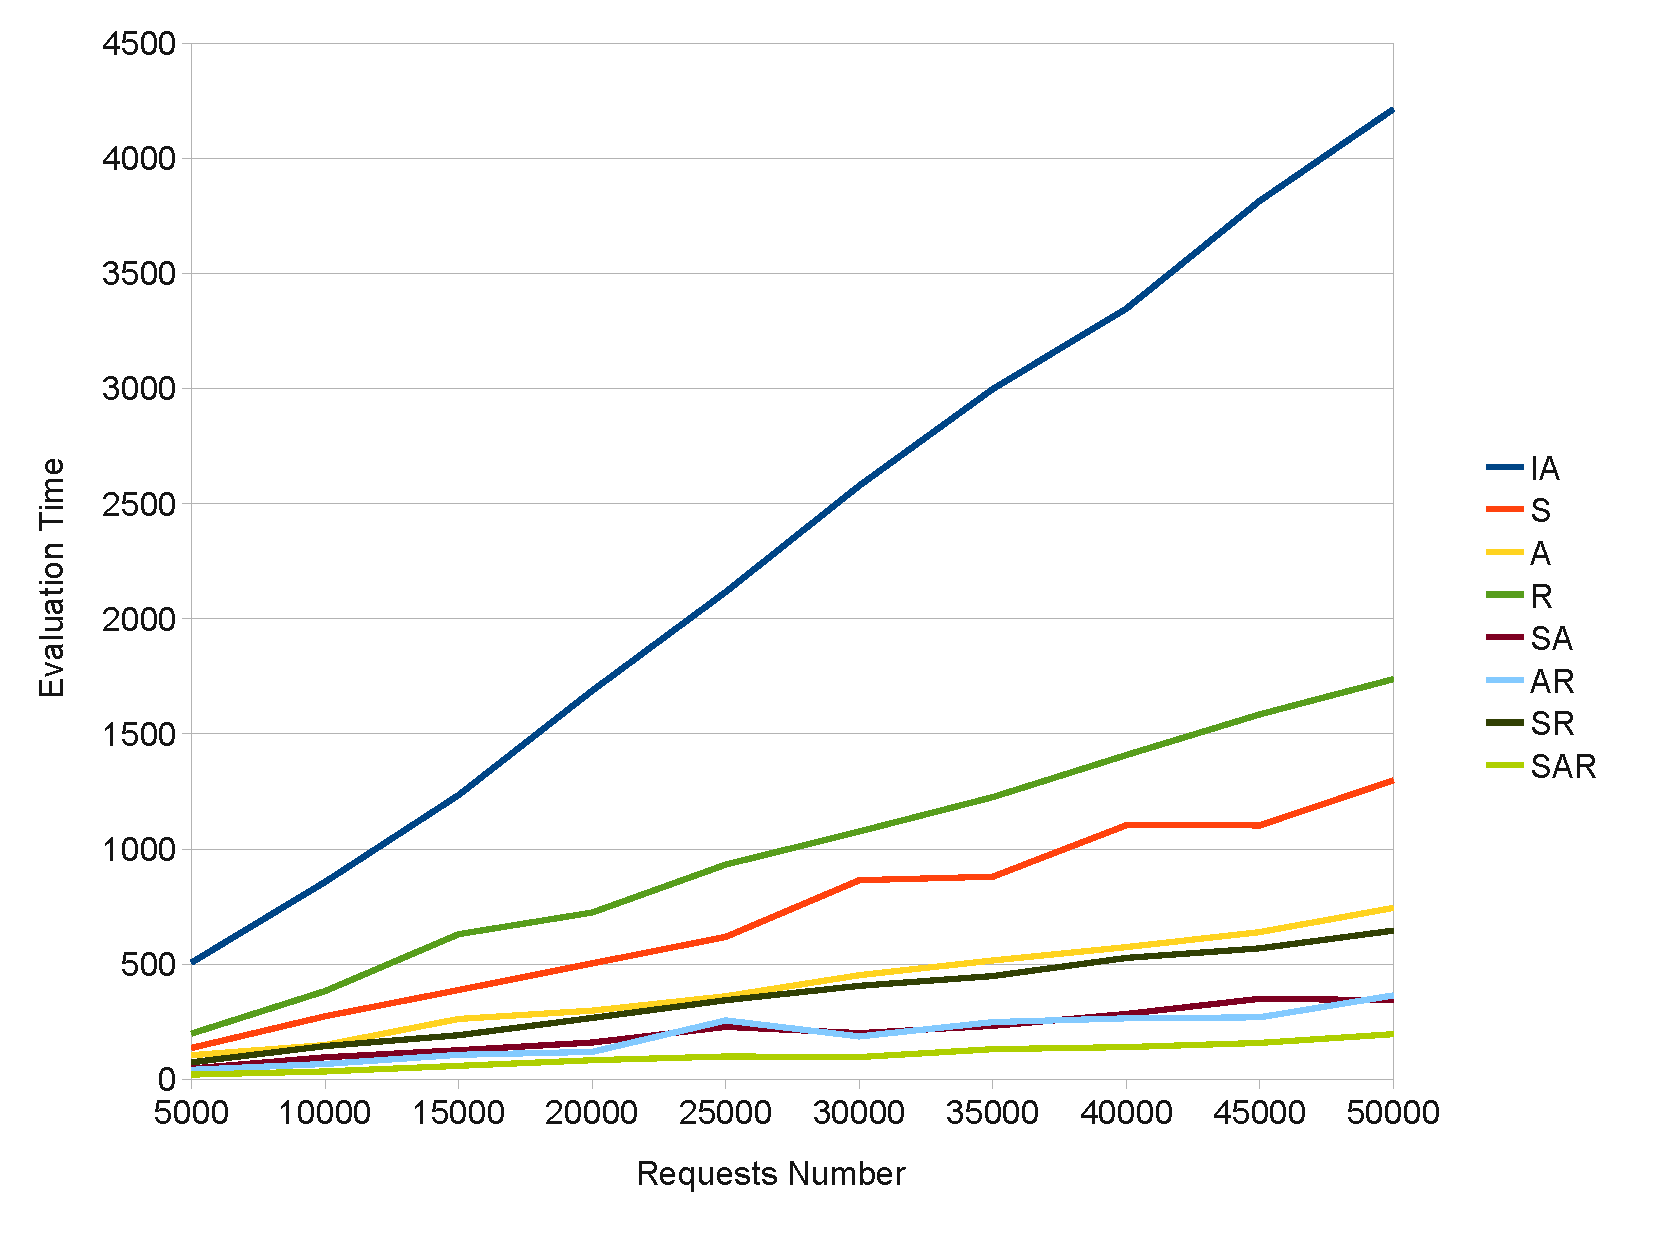
\includegraphics[width=0.33\textwidth]{X-VMS.pdf}}
  \subfloat[ASMS]{\label{fig:ASMS}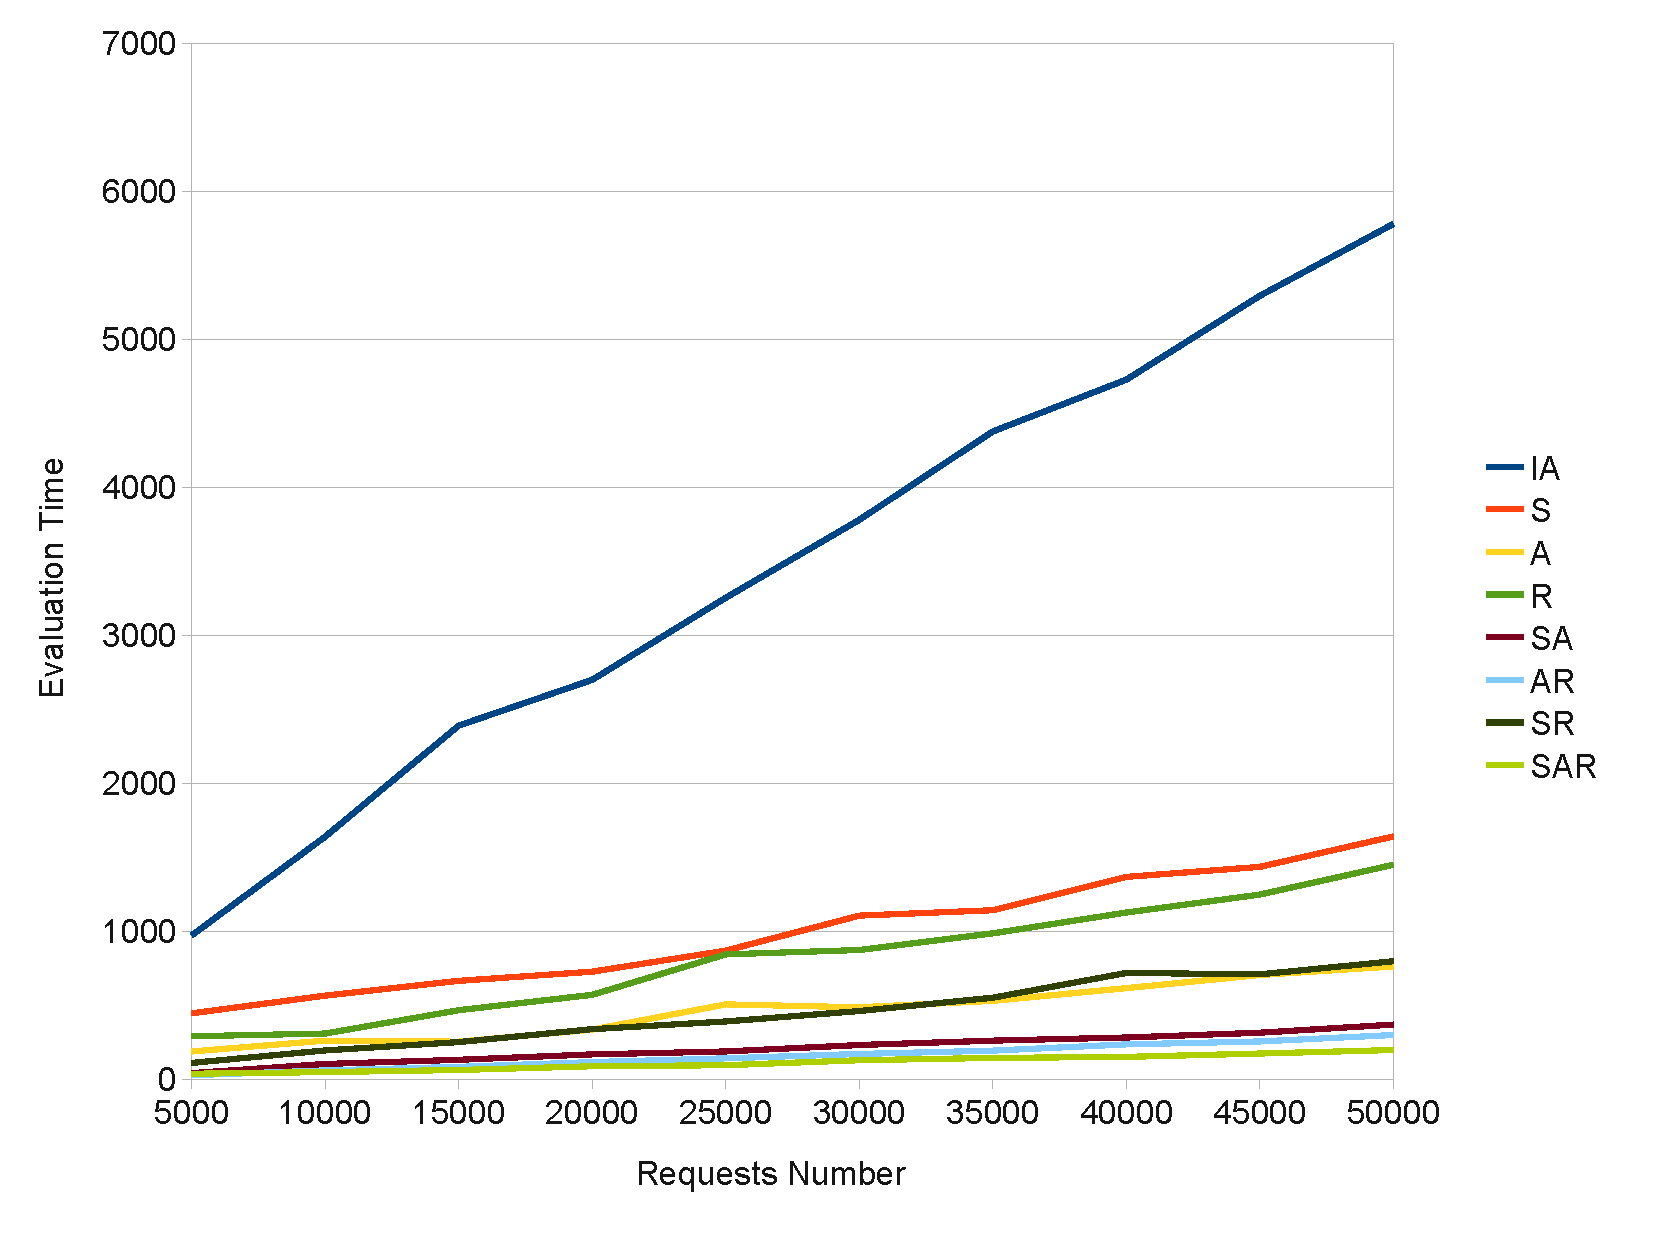
\includegraphics[width=0.33\textwidth]{X-ASMS.pdf}}
  \caption{Processing Time for our 3 systems LMS, VMS and ASMS depending on the requests Number}
  \label{fig:processing time}
\end{figure*}
We have also calculated the pourcentage of the fetching time by considering the global time of request evaluation in LMS system.
The results are shown in Table 5. This time varies between 0 and 28.6\%.

\begin{table*}[t]
\centering
\begin{tabular}{|l|l|l|l|l|l|l|l|l|l|l|}   
\hline  \rowcolor{black} \scriptsize \bf \textcolor {white}{ Requests Number (LMS)}
& \scriptsize \bf \textcolor {white}{5000}
& \scriptsize \bf \textcolor {white}{10000}
& \scriptsize \bf \textcolor  {white}{15000}
& \scriptsize \bf \textcolor  {white}{20000}
& \scriptsize \bf \textcolor  {white}{25000}
& \scriptsize \bf \textcolor  {white}{30000} 
& \scriptsize \bf \textcolor  {white}{35000}
& \scriptsize \bf \textcolor  {white}{40000}
& \scriptsize \bf \textcolor  {white}{45000}
& \scriptsize \bf \textcolor {white}{50000}\\ \hline

\scriptsize  {S }
& \scriptsize  {1.31}
& \scriptsize {0.64}
& \scriptsize {0.91}
& \scriptsize {1.01}
& \scriptsize {1.09}
& \scriptsize {1.14}
& \scriptsize {1.16}
& \scriptsize {1.03}
& \scriptsize {0.07}
& \scriptsize {1.08}
\\ \hline

\scriptsize  {A }
& \scriptsize  {1.66}
& \scriptsize {1.70}
& \scriptsize {1.71}
& \scriptsize {1.70}
& \scriptsize {1.36}
& \scriptsize {1.42}
& \scriptsize {1.47}
& \scriptsize {1.50}
& \scriptsize {1.55}
& \scriptsize {1.56}
\\ \hline


\scriptsize  {R}
& \scriptsize  {1.04}
& \scriptsize {1.06}
& \scriptsize {1.06}
& \scriptsize {0.80}
& \scriptsize {0.86}
& \scriptsize {0.91}
& \scriptsize {0.93}
& \scriptsize {0.82}
& \scriptsize {0.96}
& \scriptsize {0.87}
\\ \hline

\scriptsize  {SA}
& \scriptsize  {7.40}
& \scriptsize {7.69}
& \scriptsize {6.32}
& \scriptsize {6.60}
& \scriptsize {6.10}
& \scriptsize {6.32}
& \scriptsize {6.48}
& \scriptsize {6.16}
& \scriptsize {6.38}
& \scriptsize {6.31}
\\ \hline

\scriptsize  {AR}
& \scriptsize  {8.33}
& \scriptsize {6.12}
& \scriptsize {6.94}
& \scriptsize {7.29}
& \scriptsize {7.56}
& \scriptsize {7.09}
& \scriptsize {6.74}
& \scriptsize {6.80}
& \scriptsize {6.94}
& \scriptsize {6.66}
\\ \hline

\scriptsize  {SR}
& \scriptsize  {2.27}
& \scriptsize {3.40}
& \scriptsize {3.81}
& \scriptsize {3.40}
& \scriptsize {3.68}
& \scriptsize {3.83}
& \scriptsize {3.61}
& \scriptsize {3.73}
& \scriptsize {3.79}
& \scriptsize {3.68}
\\ \hline


\scriptsize  {SAR}
& \scriptsize {14.28}
& \scriptsize {19.23}
& \scriptsize {21.05}
& \scriptsize {19.23}
& \scriptsize {17.64}
& \scriptsize {18.98}
& \scriptsize {18.08}
& \scriptsize {18.69}
& \scriptsize {18.33}
& \scriptsize {18.97}
\\ \hline
\end{tabular}

\caption{Percentage of Fetching Time}\end{table*}


\section{Related Work} \label{sec:related}

There are several previous work about performance issues in security mechanisms.
Ammons et al.\cite{largesystems} have presented techniques to reduce the overhead engendered from implementing a security model 
in IBM's WebSphere Application Server (WAS). Their approach identifies bottlencks through code instrumentation and focuses on two aspects: the temporal redundancy (when security checks are made frequently) and the spatial redundancy
(using same security techniques on same code execution paths).
For the first aspect, they use caching mechanisms to store checks results, so that the decision is retrieved from the cache.
For the second aspect they used a technique based on specialization, which consists in replacing an expensive check with a cheaper one for frequent codes paths.
While this previous approach focus on bottlencks in program code, in this paper, we propose a new approach to refactor access control policies by reducing the number of rules in each split policy.

Various techniques \cite{MyABDAC, clustering, decomposition} have been proposed to address performance issues in systems interacting with access control policies. 
Jahid et al. \cite{MyABDAC} focus on XACML
policy verification for database access control. They presented a model, which converts attribute-based policies into access control lists. They implemented their approach, called MyABDAC.
While they measure performance on MyABDAC in terms of request evaluation, however, they do not show how much MyABDAC
gains improvement over an existing PDP.


Marouf et al. \cite{clustering} have proposed an approach for policy evaluation based on a 
clustering algorithm that reorders rules and policies within the policy set so that the access to applicable policies is faster, their categorization is based on
 the subject target element. Their technique requires identifying the rules that are frequently used. Our approach follows a different strategy and does not require knowing which 
rules are used the most. In addition, the rule reordering is tightly related to specific systems. If the PDP is shared between several
 systems, their approach could not be applicable since the most ``used'' rules may vary between systems. \\


Lin et al. \cite{decomposition} decomposed the global XACML policy into local policies related to collaborating parties, the local policies 
are sent to corresponding PDPs. The request evaluation is based on local policies by considering the relationships among local
 policies. In their approach, the optimization is based on storing the effect of each rule and each local policy for 
a given request. Caching decisions results are then used to optimize evaluation time for an incoming request. However the authors have 
not provided experimental results to measure the efficiency of their approach when compared to the traditional architecture.  
While the previous approaches have focused on the PDP component to optimize the request evaluation, Miseldine et al. \cite{XACMLstructure} addressed this problem by 
analyzing rule location on XACML policy and requests at design level so that the relevant rules for the request are accessed faster on evaluation time. 


The current contribution brings new dimensions over our previous work on access control \cite{Xengine, testcase, models}.
We have proposed XEngine \cite{Xengine}, which focuses particularly on performance issues addressed with XACML policies evaluation. XEngine proposes an 
alternative solution to brute force searching based on an XACML policy conversion to a tree structure to minimize the request evaluation time. 
It involves a refactoring process that transforms the global policy to a decision diagram that is then converted to 
forwarding tables. In this current contribution, we introduce a new refactoring process that involves splitting the policy into smaller sub-policies. Our 
two refactoring processes are combined to decrease dramatically the evaluation time. 

\section{Conclusion and Future Work} \label{sec:conclusion}

In this paper, we have tackled the performance issue in access control decision making mechanism.
We have proposed an
 automated refactoring  process  
that enables to reduce request evaluation time.
Our approach has been applied on three JAVA projects interacting with XACML policies.
To support and automate the refactoring process, we have designed and implemented a tool, called PolicySplitter,
which transforms a given policy into multiple policies according to a chosen splitting criterion.

Our evaluation results have shown that our approach gain a significant performance improvement
in terms of request evaluation time.
Our evaluation results have shown that our proposed approach
preserves the initial architectural model of the subjects in terms of interaction between the business logic and its corresponding
rules in the policy. Our evaluation results have shown that our approach
is efficient in terms of reducing request evaluation time by up to nine times. 

% The best gain in performance is reached by
%the criterion that respects the synergy property. This plead in favor of a refactoring process that takes into
% account, the way PEPs are scattered inside the system business logic. 
%In this work, we have easily identified the different PEPs since we know exactly how our system functions are
% implemented and thus how PEPs are organized inside the system.

%In our future work, we plan to develop an approach to automatically identify PEPs. 
%This technique is an important step that is complementary to this paper approach, since it enables
% knowing how PEPs are organized in the system and thus allows to select the most 
%suitable splitting criterion for a given application. 
% and it can be generalized to policies in other policy specification
%languages (such as EPAL). 


\bibliographystyle{abbrv}
\bibliography{sigproc} 
\balancecolumns


%\bibliographystyle{abbrv}
%\bibliography{sigproc} 
% That's all folks!
\end{document}
